\chapter{The Method of Integral Equations}\label{chap2}

\section{A Theorem on Balls}\label{chap2:sec1}

Let\pageoriginale $\uub{p}_{1}, \ldots, \uub{p}_{N},$ be points in $U^{k}$, all of whose coordinates are less than $1$. A point $\uub{\ell}$ in k-dimensional space $R^{k}$ will be called an {\em integer point} if all its coordinates are integers. Integer points will be denoted by $\uub{\ell}, \uub{\ell}_{1}, \uub{\ell}_{2}, \ldots$. Denote by $\mathscr{P}$ the set of points $\uub{p}_{i} + \uub{\ell}$, $1 \leq i \leq n$, where $\uub{\ell}$ runs over all the integer points. Thus $\mathscr{P}$ is a ``periodic'' set. Let $A$ be a bonded set with volume $\mu(A)$. Write
$$
z(A) \text{ for the number of points of } \mathscr{P} \text{ in }A,
$$
and 
$$
D(A) = z(A) - N\mu(A).
$$

Call $D(A)$ the `error'. Let $K(r, \uub{c})$ be the ball with radius $r$ and centre $\uub{c}$, i. e. the set of all the points $\uub{x}$ with $|\uub{x} - \uub{c}| \leq r$. Put
$$
z(r, \uub{c}) = z(K(r, \uub{c})), D(r, \uub{c}) = D(K(r, \uub{c})), \mu(r) = \mu(K(r, \uub{c})).
$$ 

Set
$$
E(r, s) = \int_{U^{k}} D(r, \uub{c}) D(s, \uub{c}) d\uub{c}.
$$

\begin{theorem}[~(W. M. Schmidt \cite{22})]\label{chap2:sec1:thm1A}
 Let $k > 0$, $\epsilon > 0$. Suppose $\delta > 0$ satisfies $N \delta^{k} > N^{\epsilon}$. Then
$$
\int_{0}^{\delta} r^{-1} E(r, r)dr \gg (n \delta^{k})^{1 - \dfrac{1}{k} - \epsilon},
$$
where the constant implied by $\gg$ depends on $k$ and $\epsilon$, but is independent of $N$ and $\delta$.
\end{theorem}

\begin{theorem}\label{chap2:sec1:thm1B}
Let $k, \in, \delta$ be as in Theorem 1\ref{chap2:sec1:thm1A}. Then there exists a ball $K(r, \uub{c})$ with $r \leq \delta$ and
$$
|D(r, \uub{c})| \gg (n \delta^{k})^{\frac{1}{2} - \frac{1}{2k} - \epsilon},
$$\pageoriginale
where the constant implied by $\gg$ depends on $k$ and $\epsilon$, but is independent of $N$ and $\delta$.
\end{theorem}

According to Theorem 1\ref{chap2:sec1:thm1B}, there exists a ball with `error' very large as compared with that of boxes with sides parallel to the axes. We recall: Roth proved (see Chapter I, \S\ \ref{chap1:sec2}), that there exists a box $B$ with sides parallel to the axes contained in $U^{k}$ with
$$
|D(B)| > c (\log N)^{\frac{k-1}{2}}.
$$ 

On the other hand, there are distributions of $N$ points such that $|D(B)| < c' (\log N)^{k-1}$ (see Chapter I, \S\ \ref{chap1:sec2}).

\medskip
\begin{remarks*}
~
 \begin{enumerate}[(i)]
  \item If $\delta$ and $k$ are fixed, the hypotheses of Theorem 1\ref{chap2:sec1:thm1A} and Theorem 1\ref{chap2:sec1:thm1B} are satisfied for large $N$. On the other hand, we can allow $\delta$ to be small, namely as small as $\delta^{k} = N^{-1+2\epsilon}$, and still we get a lower bound which tends to infinity with $N$.
  \item The ball $K(r, \uub{c})$ of Theorem 1\ref{chap2:sec1:thm1B} is not necessarily contained in $U^{k}$.
 \item One would like to ask if there exists a ball with positive $D(r, \uub{c})$ and with
$$
D(r, \uub{c}) \gg (N \delta^{k})^{\frac{1}{2} - \frac{1}{2k} - \epsilon},
$$
or a ball with negative $D(r, \uub{c})$ and with
$$
-D(r, \uub{c}) \gg (N \delta^{k})^{\frac{1}{2} - \frac{1}{2k} - \epsilon}.
$$
 \item We do not know what would be the best possible exponent in the estimate of Theorem 1\ref{chap2:sec1:thm1B}, Using probabilistic methods, one sees the existence of points $\uub{p}_{1}, \ldots, \uub{p}_{N}$ with
$$
|D(r, \uub{c})| \ll N^{\frac{1}{2} + \epsilon}, \text{ if } r \leq 1.
$$
 \end{enumerate}
\end{remarks*}

(See,\pageoriginale e.g., W. Philipp \cite{18}.)

\medskip
\noindent{\textit{We shall prove that Theorem 1\ref{chap2:sec1:thm1A} implies Theorem 1\ref{chap2:sec1:thm1B}.}} For this we require the following:
\begin{lemma}\label{chap2:sec1:lem1C}
$$
|E(r, s)| \ll N^{2} \max (r^{k} s^{k}, \min (r^{k}, s^{k})).
$$
\end{lemma}

\begin{remark*}
Here and later, the constant in $\ll$ depends on $k$ and $\epsilon$, but is independent of $n, \delta$.
\end{remark*}

\begin{proof}
Note that
$$
|E(r, s)| \leq \int_{U^{k}} (z(r, \uub{c}) + N\mu(r))(z(s, \uub{c}) + N\mu(s))d \uub{c}.
$$
\end{proof}

Observe that
\begin{align*}
z(s, \uub{c}) & \ll N \max (1, s^{k}),\\
\int_{U^{k}} z(s, \uub{c}) d \uub{c} & = N\mu(s) \ll N s^{k}.\tag{1.1}\label{chap2:sec1:eq1.1} 
\end{align*}

Using these relations, we obtain
\begin{align*}
|E(r, s)| & \ll N \max (1, r^{k}) \int_{U^{k}} (z(s, \uub{c}) + N\mu(s)) d \uub{c}\\
& \ll N \max (1, r^{k}) N s^{k}\\
& = N^{2} \max (s^{k}, r^{k} s^{k}).
\end{align*}

Since $|E(r, s)|$ is symmetric in $r$ and $s$, we also obtain
$$
|E(r, s)| \ll N^{2} \max (r^{k}, r^{k} s^{k}).
$$

Hence
$$
|E(r, s)| \ll N^{2} \max (r^{k} s^{k}, \min (r^{k}, s^{k})).
$$

This proves Lemma 1\ref{chap2:sec1:lem1C}.

The\pageoriginale proof that Theorem 1\ref{chap2:sec1:thm1A} implies Theorem 1\ref{chap2:sec1:thm1B} runs as follows. If $N \delta^{k} \ll 1$, take a ball with centre $\uub{p}_{i}$ and very small radius $r$. Then
\begin{align*}
|D(r, \uub{c})| & \geq |z(r, \uub{c})| - |N\mu(r)|\\
& \geq 1 - \frac{1}{2} = \frac{1}{2} \gg (N \delta^{k})^{\frac{1}{2} - \frac{1}{2k} - \epsilon}.
\end{align*}

So we may assume that $N \delta^{k} > c'$, where $c'$ is a large positive constant depending only on $k$ and $\epsilon$. Put
$$
\eta = N^{-2/k}
$$

Then $\eta < \delta$, since $N \eta^{k} = N^{-1} \leq N^{\epsilon} < N \delta^{k}$. By Lemma 1\ref{chap2:sec1:lem1C},
\begin{equation*}
\int_{0}^{\eta} r^{-1} E(r, r)dr \ll N^{2} \int_{0}^{\eta} r^{k-1} dr \gg N^{2} \eta^{k} = 1.\tag{1.2}\label{chap2:sec1:eq1.2}
\end{equation*}

From Theorem 1\ref{chap2:sec1:thm1A} and (\ref{chap2:sec1:eq1.2}), we obtain
\begin{equation*}
\int_{\eta}^{\delta} r^{-1} E(r, r)dr \gg (N \delta^{k})^{1 - \frac{1}{k} - \epsilon},\tag{1.3}\label{chap2:sec1:eq1.3}
\end{equation*}
if $c'$ is large enough. Notice that
\begin{equation*}
\left|\int_{\eta}^{\delta} r^{-1} E(r, r) dr\right| \leq (\max_{\eta \leq r \leq \delta} |E(r, r)|) \int_{\eta}^{\delta} r^{-1} dr.\tag{1.4}\label{chap2:sec1:eq1.4}  
\end{equation*}

But
\begin{align*}
\int_{\eta}^{\delta} r^{-1} dr = \log (\frac{\delta}{\eta}) & = \log (\delta N^{2/k})\\
 & = \frac{1}{k} \log (\delta^{k} N, N)\\
 & \ll \log (\delta^{k} N) \ll (\delta^{k} N)^{\epsilon}\tag{1.5}\label{chap2:sec1:eq1.5}
\end{align*}
since $\delta^{k} N > N^{\epsilon}$ and since $N \delta^{k}$ is large. Combining $(1.3), (1.4), (1.5)$, we conclude that there is an $r$ with $\eta \leq r \leq \delta$ and 
$$
|E(r, r)| \gg (N \delta^{k})^{1 - \frac{1}{k} - \epsilon}.
$$

Hence there exists a $\uub{c} \in U^{k}$ such that
$$
|D(r, \uub{c})| \gg (N \delta^{k})^{\frac{1}{2} - \frac{1}{2k} - \frac{\epsilon}{2}}.
$$\pageoriginale

Thus Theorem 1\ref{chap2:sec1:thm1B} is true.

\section{Setting up an Integral Equation}\label{chap2:sec2}

Let $k$ be an integer $> 1$. Put
\begin{equation*}
 \nu = 
 \begin{cases}
  1, & \text{ if } k \text{ is odd },\\
  0, & \text{ if } k \text{ is even}. 
 \end{cases}
\end{equation*}

Let $0 < \alpha < 1$, and let $\beta$ be such that $\alpha + \beta = 1 + \nu$. Assume that $\delta > 0$. Put
$$
A = \mathop{\int_{0}^{1} \int_{0}^{1}}_{r+s \leq 1} E(\delta r, \delta s) |r-s|^{-\alpha} |r+s|^{-\beta} dr \quad ds.
$$

We shall show that
\begin{equation*}
|A| \ll \int_{0}^{\delta} E(r, r) r^{-1} dr,\tag{2.1}\label{chap2:sec2:eq2.1}
\end{equation*}
where the constant implied by $\ll$ depends only on $\alpha$ and $k$. Note that
\begin{align*}
|2E(r, s)| & \leq \int_{U^{k}} 2|D(r, \uub{c}) D(s, \uub{c})|d \uub{c}\\
& \leq \int_{U^{k}} (D^{2} (r, \uub{c}) + D^{2}(s, \uub{c})) d \uub{c}\\
& = E(r, r) + E(s, s).
\end{align*}

Therefore
$$
|A| \leq \frac{1}{2} \mathop{\int_{0}^{1} \int_{0}^{1}}_{r+s \leq 1} (E(\delta r, \delta r) + E(\delta s, \delta s)) |r-s|^{-\alpha} |r+s|^{-\beta} dr \quad ds.
$$

Since $|r-s|^{-\alpha} |r+s|^{-\beta}$ is symmetric in $r$ and $s$, we have
\begin{align*}
|A| & \leq \mathop{\int_{0}^{1} \int_{0}^{1}}_{r+s \leq 1} E(\delta r, \delta r) |r-s|^{-\alpha} |r+s|^{-\beta} dr \quad ds\\
& = \int_{0}^{1} E(\delta r, \delta r)r^{-\nu} dr \int_{0}^{\frac{1}{r} - 1} |1 - t|^{-\alpha} |1 + t|^{-\beta} dt,
\end{align*}
by\pageoriginale introducing a new variable $t$ given by $s = rt$. For $0 < r \leq 1$, observe that the inner integral 
\begin{equation*}
\int_{0}^{\frac{1}{r} - 1} |1 - t|^{-\alpha} |1 + t|^{-\beta} dt \ll
 \begin{cases}
  1, & \text{ if } \alpha + \beta = 1 + \nu = 2,\\
  1, & \text{ if } 1 + \nu < 2 \text{ and } \frac{1}{r} \leq 10,\\
  \log \frac{1}{r}, & \text{ if } 1 + \nu = 1 \text{ and } \frac{1}{r} > 10.
 \end{cases}
\end{equation*}

So in general the above integral is
$$
\ll (1 + \log \frac{1}{r})^{1-\nu} \ll r^{\nu -1} \qquad (0 < r \leq 1).
$$

Hence 
$$
|A| \ll \int_{0}^{1} E(\delta r, \delta r) r^{-1} dr = \int_{0}^{\delta} E(r, r) r^{-1} dr,
$$
and (\ref{chap2:sec2:eq2.1}) is proved.

Put 
\begin{equation*}
f(r, \uub{c}; \uub{x}) = 
 \begin{cases}
  1, & \text{ if } \uub{x} \epsilon K(r, \uub{c}),\\
  0 & \text{ otherwise },
 \end{cases}
\end{equation*}
so that $f(r, \uub{c} ; \uub{x})$ for fixed $r, \uub{c}$ is the characteristic function of $K(r, \uub{c})$.

Write
$$
g(r, \uub{c} ; \uub{x}) = \sum_{\uub{\ell}} f(r, \uub{c} ; \uub{x} + \ell),
$$
where the sum is taken over all the integer points $\ell$. Notice that $f(r, \uub{c} ; \uub{x} + \uub{\ell}) = 0$ except for finitely many $\uub{\ell}$. Further observe that
\begin{equation*}
z(r, \uub{c}) = \sum_{i=1}^{N} \sum_{\uub{\ell}} f(r, \uub{c} ; \uub{p}_{i} + \uub{\ell}) = \sum_{i=1}^{N} g(r, \uub{c} ; \uub{p}_{i}).\tag{2.2}\label{chap2:sec2:eq2.2}
\end{equation*}

Put
$$
\omega (\uub{x}, \uub{y}) = \min_{\uub{\ell}} |\uub{x} - \uub{y} - \uub{\ell}|.
$$
where the minimum is taken over all the integer points. We could interpret $\omega$ as the ``distance modulo $1$'' of $\uub{x}$ and $\uub{y}$. Denote by $K(r, s, \omega)$ the volume of\pageoriginale the intersection of two balls with radii $r$ and $s$, whose centres have distance $\omega$. {\em We shall show that if $r$ and $s$ are positive real numbers with $r + s < \dfrac{1}{2}$, then}
\begin{equation*}
E(r, s) = \sum_{i=1}^{N} \sum_{j=1}^{N} (K(r, s, \omega) (\uub{p}_{i}, \uub{p}_{j})) - \int_{U^{k}} \int_{U^{k}} K(r, s, \omega (\uub{x}, \uub{y}) d\uub{x} \quad d\uub{y}).\tag{2.3}\label{chap2:sec2:eq2.3}
\end{equation*}

We start by noting that
\begin{align*}
E(r, s) & = \int_{U^{k}} D(r, \uub{c}) D(s, \uub{c}) d\uub{c}\\
 & = \int_{U^{k}} (z(r, \uub{c}) -N\mu(r)) (z(s, \uub{c}) - N\mu (s)) d\uub{c}\\
 & = \int_{U^{k}} (z(r, \uub{c}) z(s, \uub{c})) d\uub{c} - N^{2} \mu (r) \mu (s)\tag{2.4}\label{chap2:sec2:eq2.4}
\end{align*}
since
{\fontsize{10}{12}\selectfont
$$
\int_{U^{k}} z(r, \uub{c}) d\uub{c} = \sum_{i=1}^{N} \sum_{\uub{\ell}}
\int_{U^{k}} f(r, \uub{c} - \uub{\ell} ; \uub{p}_{i}) d\uub{c} =
\sum_{i=1}^{N} \int_{R^{k}} f(r, \uub{c} ; \uub{p}_{i})d\uub{c} =
N\mu(r). 
$$}\relax

From (\ref{chap2:sec2:eq2.2}) and (\ref{chap2:sec2:eq2.4}),
\begin{equation*}
E(r, s) = \sum_{i=1}^{N} \sum_{j=1}^{N} (\int_{U^{k}} g(r, \uub{c} ; \uub{p}_{i}) g(s, \uub{c} ; \uub{p}_{i}) d\uub{c} - \mu(r) \mu(s))\tag{2.5}\label{chap2:sec2:eq2.5}
\end{equation*}

The integral
$$
\int_{U^{k}} g(r, \uub{c} ' \uub{x}) g(s, \uub{c} ; \uub{y}) d\uub{c}
$$
is periodic in $\uub{x}$ and $\uub{y}$. (That is, the integral remains unchanged if $\uub{x}$ and $\uub{y}$ are replaced by $\uub{x} + \uub{\ell}_{1}$ and $\uub{y} + \uub{\ell}_{2}$, respectively). Therefore to study the integral we may assume that $\uub{x} = (x_{1}, \ldots, x_{k})$, $\uub{y} = (y_{1}, \ldots, y_{k})$ satisfy $|x_{i} - y_{i}| \leq \dfrac{1}{2} (1 \leq i \leq k)$. Observe that
\begin{align*}
\int_{U^{k}} g(r, \uub{c} ; \uub{x}) g(s, \uub{c} ; \uub{y}) d\uub{c} & = \int_{U^{k}} \sum_{\uub{\ell}_{1}} \sum_{\uub{\ell}_{2}} f(r, \uub{c} -\uub{\ell}_{1} ; \uub{x}) f(s, \uub{c} - \uub{\ell}_{2} ; \uub{y}) d\uub{c}\\
& = \sum_{\uub{\ell}} \int_{U^{k}} f(r, \uub{c} - \uub{\ell} ; \uub{x}) f(s, \uub{c} - \uub{\ell} ; \uub{y}) d\uub{c},
\end{align*}
since\pageoriginale if $\uub{\ell}_{1} = (\ell_{11}, \ldots, \ell_{1k})$, $\uub{\ell}_{2} = (\ell_{21}, \ldots, \ell_{2k})$, $\uub{c} = (c_{1}, \ldots, c_{k})$ and $f(r, \uub{c} - \uub{\ell}_{1} ;  \uub{x}) = f(s, \uub{c} - \uub{\ell}_{2} ; \uub{y}) = 1$, then
$$
|c_{i} - \ell_{1i} - x_{i}| \leq r \text{ and } |c_{i} - \ell_{2i} - y_{i}| \leq s \qquad (1 \leq i \leq k).
$$

So $|\ell_{1i} - \ell_{2i}| \leq r+s+|x_{i}-y_{i}|< \dfrac{1}{2} + \dfrac{1}{2} = 1 \quad (1 \leq i \leq k)$. which implies that $\ell_{1i} = \ell_{2i}$ for $1 \leq i \leq k$, i.e. that $\uub{\ell}_{1} = \uub{\ell}_{2}$. Therefore
\begin{align*}
\int_{U^{k}} g(r, \uub{c} ; \uub{x}) g(s, \uub{c} ; \uub{y}) d\uub{c} & = \int_{R^{k}} f(r, \uub{c} ; \uub{x}) f(s, \uub{c} ; \uub{y}) d\uub{c}\\
& = K(r, s, |\uub{x} - \uub{y}|).
\end{align*}

This holds if $|x_{i} - y_{i}| \leq \dfrac{1}{2} (1 \leq i \leq k).$ In general we have
\begin{equation*}
\int_{U^{k}} g(r, \uub{c} ; \uub{x}) g(s, \uub{c} ; \uub{y}) d\uub{c} = K(r, s, \omega(\uub{x}, \uub{y}))\tag{2.6}\label{chap2:sec2:eq2.6}
\end{equation*}

The last equation yields
\begin{align*}
\int_{U^{k}} \int_{U^{k}} & K(r, s, \omega(\uub{x}, \uub{y})) d\uub{x} \quad d\uub{y}\\ 
& = \int_{U^{k}} \int_{U^{k}} \int_{U^{k}} g(r, \uub{c} ; \uub{x}) g(s, \uub{c} ; \uub{y}) d\uub{c} \quad d\uub{x} \quad d\uub{y}\\
& = \int_{U^{k}} (\int_{U^{k}} g(r, \uub{c} ; \uub{x}) (d\uub{x}) (\int_{U^{k}} g(s, \uub{c} ; \uub{y}) d\uub{y}) d\uub{c}\\
& = \mu (r) \mu (s)\tag{2.7}\label{chap2:sec2:eq2.7}
\end{align*}
since $\int_{U^{k}} g(r, \uub{c} ; \uub{x}) d \uub{x} = \sum_{\uub{\ell}} \int_{U^{k}} f(r, \uub{c} ; \uub{x} + \uub{\ell}) dx = \int_{R^{k}} f(r, \uub{c} ; \uub{x}) = \mu(r)$.

Combining (\ref{chap2:sec2:eq2.5}), (\ref{chap2:sec2:eq2.6}) and (\ref{chap2:sec2:eq2.7}), we obtain (\ref{chap2:sec2:eq2.3}).

\begin{lemma}[ (Fundamental Lemma)]\label{chap2:sec2:lem2A}
Suppose that $0 < \delta < \dfrac{1}{2}$. Suppose $f(r)$ is continuous in $0 < r \leq \dfrac{1}{2}$ with
$$
|f(r)| \ll r^{1-k-\alpha} \text{ as } r \to 0,
$$
and satisfies the integral equation
\begin{equation*}
\int_{0}^{\frac{1}{2}} K(r\delta, r\delta, \omega)f(r) dr = \mathop{\int_{0}^{1} \int_{0}^{1}}_{r+s \leq 1} \frac{K(r\delta, s\delta, \omega)}{|r-s|^{\alpha} |r+s|^{\beta}}dr \quad ds \quad (\omega \leq 0).\tag{2.8}\label{chap2:sec2:eq2.8}
\end{equation*}
\end{lemma}

Then\pageoriginale
\begin{equation*}
\int_{0}^{\frac{1}{2}} E(\delta r, \delta r) f(r) dr = \int_{0}^{1} \int_{0}^{1} \frac{E(\delta r, \delta s)}{|r - s|^{\alpha} |r+s|^{\beta}}. dr \quad ds.\tag{2.9}\label{chap2:sec2:eq2.9}
\end{equation*}

\begin{proof}
The lemma follows immediately from $(2.3)$. All the functions occurring in the integrals are summable.
\end{proof}

\begin{remark*}
{\em If (\ref{chap2:sec2:eq2.8}) is true for some $\delta > 0$, then (\ref{chap2:sec2:eq2.8}) and (\ref{chap2:sec2:eq2.9}) are true for every} $\delta > 0$. This is seen as follows. For a positive integer $m$, denote by $\mathscr{P}^{*}$ the set $\dfrac{1}{m} \mathscr{P}$. Define $E^{*}(r, s)$ with reference to $\mathscr{P}^{*}$. Notice that for every $r, s > 0$,
\begin{equation*}
E^{*} \left(\frac{r}{m}, \frac{s}{m}\right) = E(r, s),\tag{2.10}\label{chap2:sec2:eq2.10}
\end{equation*}
since the set $\mathscr{P}$ is periodic and $D^{*} (\dfrac{r}{m},
\dfrac{\uub{c}}{m}) = D(r, \uub{c}), D^{*} (\dfrac{s}{m},
\dfrac{\uub{c}}{m})\break = D(s, \uub{c})$. 
\end{remark*}

Suppose that (\ref{chap2:sec2:eq2.8}) is true for some $\delta > 0$. Since for any $c > 0$, $K(cr, cs, c\omega) = c^{k} K(r, s, \omega)$, (\ref{chap2:sec2:eq2.8}) is true for $c \delta$ and hence for every $\delta > 0$. Now given $\delta > 0$, choose an integer in such that $\delta / m < \dfrac{1}{2}$. Then by Lemma 2\ref{chap2:sec2:lem2A},
$$
\int_{0}^{\frac{1}{2}} E^{*} \left(\frac{\delta}{m} r, \frac{\delta}{m}r\right) f(r) dr = \mathop{\int_{0}^{1} \int_{0}^{1}}_{r+s \leq 1} \frac{E^{*} \left(\frac{\delta}{m} r, \frac{\delta}{m} s\right)}{|r-s|^{\alpha} |r+s|^{\beta}}dr \quad ds,
$$
which along with (\ref{chap2:sec2:eq2.10}) gives (\ref{chap2:sec2:eq2.9}).

\section{Differentiating the Integral Equation}\label{chap2:sec3}

\label{64}
In view of the Remarks at the end of \S\ \ref{chap2:sec2}, we may restrict ourselves to the equation (\ref{chap2:sec2:eq2.8}) with $\delta = 1$, i. e. to 
\begin{equation*}
\int_{0}^{\frac{1}{2}} f(r) K(r, r, \omega) dr = \mathop{\int_{0}^{1} \int_{0}^{1}}_{r+s \leq 1} \frac{K(r, s, \omega)}{|r-s|^{\alpha} |r+s|^{\beta}}dr \quad ds \quad (\omega \geq 0).\tag{3.1}\label{chap2:sec3:eq3.1}
\end{equation*}

We shall determine a solution $f(r)$ of this integral equation. It is sufficient to consider (\ref{chap2:sec3:eq3.1}) for $0 \leq \omega < 1$, since both sides of (\ref{chap2:sec3:eq3.1}) are zero when $\omega \geq 1$.

Further\pageoriginale we may assume that $0 < \omega < 1$, since both sides of (\ref{chap2:sec3:eq3.1}) are continuous functions of $\omega$. In fact they satisfy a Lipschitz condition, since
\begin{equation*}
|K(r, s, \omega) - K(r, s, \omega')| \ll |\omega - \omega'| \min (r^{k-1}, s^{k-1}),\tag{3.2}\label{chap2:sec3:eq3.2}
\end{equation*}
since
\begin{equation*}
\int_{0}^{\frac{1}{2}} |f(r)| r^{k-1} dr \ll 1\tag{3.3}\label{chap2:sec3:eq3.3}
\end{equation*}
by virtue of $f(r) \ll r^{1-k-\alpha}$, and since
\begin{equation*}
\mathop{\int_{0}^{1} \int_{0}^{1}}_{r+s \leq 1} \frac{\min (r^{k-1}, s^{k-1})}{|r-s|^{\alpha} |r+s|^{\beta}} dr \quad ds \ll 1.\tag{3.4}\label{chap2:sec3:eq3.4}
\end{equation*}

Now suppose that $|r-s| < \omega < r+s$. Let $K(r, \uub{c})$, $K(s, \uub{d})$ be balls with $|\uub{c} - \uub{d}| = \omega$. The boundaries of $K(r, \uub{c})$, $K(s, \uub{d})$ intersect in a sphere $S^{k-2}$. Denote the radius of $S^{k-2}$ by $e$, the distance from the centre of $S^{k-2}$ to $\uub{c}$, $\uub{d}$ by $a, b$, respectively. (The reader might want to draw a sketch). We have
$$
a+b = \omega, a^{2} + e^{2} = r^{2} \text{ and } b^{2} + e^{2} = s^{2}.
$$

Eliminating $a$ and $b$, we obtain
$$
e^{2} = \frac{1}{4} (1 -\frac{(r-s)^{2}}{\omega^{2}}) ((r+s)^{2} - \omega^{2}).
$$

We have
$$
K(r, s, \omega) = c_{1} \int_{0}^{e} z^{k-2} (\sqrt{r^{2} - z^{2}} + \sqrt{s^{2} - z^{2}} - \omega)dz.
$$

(The constant $c_{1}$ and subsequent constants $c_{2}, c_{3}, \ldots$ are positive and depend only on $k$ and on $\alpha$). Since the integrand vanishes for $z = e$, we obtain
$$
\frac{\partial}{\partial \omega} K(r, s, \omega) = -c_{1} \int_{0}^{e} z^{k-2} dz = -c_{2} e^{k-1}.
$$\pageoriginale

All this holds for $|r-s| < \omega < |r+s|$. For $\omega \leq |r-s|$, $K(r, s, \omega)$ is independent of $\omega$, and for $\omega \geq r+s$, we have $K(r, s, \omega) = 0$. From all this, it follows that 
\begin{equation*}
\frac{\partial}{\partial \omega} K(r, s, \omega) =
 \begin{cases}
  -c_{2} e^{k-1} & \text{ if } |r-s|< \omega < r+s,\\
   0 & \text{ otherwise }.
 \end{cases}
\end{equation*}

Now we differentiate both sides of (\ref{chap2:sec3:eq3.1}) with respect to $\omega$. By (\ref{chap2:sec3:eq3.2}), (\ref{chap2:sec3:eq3.3}) and Lebesgue's Theorem on dominated convergence, (see e.g., \S\ 19 of [14]), the left hand side of (\ref{chap2:sec3:eq3.1}) can be differentiated inside the integral. 

By (\ref{chap2:sec3:eq3.2}), (\ref{chap2:sec3:eq3.3}) and the dominated convergence Theorem, the same can be done for the right hand side of (\ref{chap2:sec3:eq3.1}). The derivative of the left hand side of (\ref{chap2:sec3:eq3.1}) is
\begin{equation*}
-c_{2} \int_{\omega/2}^{\frac{1}{2}} f(r) (r^{2} - \frac{\omega^{2}}{4})^{(k-1)/2} dr.\tag{3.5}\label{chap2:sec3:eq3.5}
\end{equation*}

The derivative of the right hand side of (\ref{chap2:sec3:eq3.1}) is
$$
-c_{2} \mathop{\int_{0}^{1} \int_{0}^{1}}_{|r-s| \leq \omega \leq r+s \leq 1} \frac{\left(\frac{1}{4}\left(1 - \frac{(r-s)^{2}}{\omega^{2}}\right) ((r+s)^{2} - \omega^{2})\right)^{(k-1)/2}}{|r-s|^{\alpha} |r+s|^{\beta}} dr \quad ds.
$$

Put $x = r+s$ and $y = |r-s|$. The above integral becomes
\begin{align*}
& -c_{3} \left(\int_{\omega}^{1} (x^{2} - \omega^{2})^{(k-1)/2} x^{-\beta} dx\right) \left(\int_{0}^{\omega} (1 - \frac{y^{2}}{\omega^{2}})^{(k-1)/2} y^{-\alpha} dy\right)\\
& = -c_{4} \omega^{1-\alpha} \int_{\omega}^{1} x^{-\beta} (x^{2} - \omega^{2})^{(k-1)/2} dx,
\end{align*}
since substituting $y = t \omega$ we get
$$
\int_{0}^{\omega} \left(1 - \frac{y^{2}}{\omega^{2}}\right)^{(k-1)/2} y^{-\alpha} dy = \omega^{1 - \alpha} \int_{0}^{1} (1 - t^{2})^{(k-1)/2} t^{-\alpha} dt.
$$

Hence after differentiation, the equation (\ref{chap2:sec3:eq3.1}) becomes
\begin{align*}
\int_{\omega/2}^{\frac{1}{2}} f(r)(r^{2} & - \frac{\omega^{2}}{4})^{(k-1)/2} dr\\ 
& = c_{5} \omega^{1- \alpha} \int_{\omega}^{1} x^{-\beta} (x^{2} - \omega^{2})^{(k-1)/2} dx \quad(o < \omega < 1).\tag{3.6}\label{chap2:sec3:eq3.6}
\end{align*}\pageoriginale

Any solution of this integral equation is also a solution of (\ref{chap2:sec3:eq3.1}), since both sides of (\ref{chap2:sec3:eq3.1}) are continuous and are zero for $\omega = 1$. Putting $\omega^{2} = t$ in (\ref{chap2:sec3:eq3.6}), we get
\begin{align*}
\int_{\frac{\sqrt{t}}{2}}^{\frac{1}{2}} f(r)& \left(r^{2}  - \frac{t}{4}\right)^{(k-1)/2} dr\\ 
& = c_{5} t^{(1-\alpha)/2} \int_{\sqrt{t}}^{1} x^{-\beta} (x^{2} - t)^{(k-1)/2} dx\, (0 < t < 1).\tag{3.7}\label{chap2:sec3:eq3.7}
\end{align*}

We now differentiate (\ref{chap2:sec3:eq3.7})
$$
m = \left[\frac{k}{2}\right] = \frac{k- \nu}{2}
$$
times with respect to $t$. The left hand side becomes
$$
c_{6} (-1)^{m} \int_{\frac{\sqrt{t}}{2}}^{\frac{1}{2}} f(r) \left(r^{2} - \frac{t}{4}\right)^{(\nu - 1)/2} dr.
$$

If on the right hand side we differentiate $t^{(1-\alpha)/2}$ precisely $i$ times, and the integral $\int_{\sqrt{t}}^{1} x^{-\beta} (x^{2} - t)^{(k-1)/2} dx$ $(m-i)$ times, we obtain
\begin{align*}
& (-1)^{m} c_{6}^{(0)} t^{(1-\alpha)/2} \int_{\sqrt{t}}^{1} x^{-\beta} (x^{2} - t)^{(\nu - 1)/2} dx\\
& = (-1)^{m} c_{6}^{(0)} \int_{1}^{1/\sqrt{t}} y^{-\beta} (y^{2} - 1)^{(\nu - 1)/2} dy \text{ if } i = 0
\end{align*}
and

\begin{align*}
& (-1)^{m} c_{6}^{(i)} t^{(1-\alpha-2i)/2} \int_{\sqrt{t}}^{1} x^{-\beta} (x^{2} - t)^{(k-1-2m)/2} dx\\
& = (-1)^{m} c_{6}^{(i)} \int_{1}^{1/\sqrt{t}} y^{-\beta} (y^{2} - 1)^{(\nu-1+2i)/2} dy \text{ if } 1 \leq i \leq m.
\end{align*}

Here all the constants $c_{6}^{(i)}$ are positive $(0 \leq i \leq m)$. Hence (\ref{chap2:sec3:eq3.7}) becomes 
\begin{align*}
& \int_{\sqrt{t/2}}^{\frac{1}{2}} f(r) (r^{2} - \frac{t}{4})^{(\nu - 1)/2} dr\\
& = c_{7}^{(0)} \int_{1}^{1/\sqrt{t}} y^{-\beta} (y^{2} - 1)^{(\nu - 1)/2} dy\\ 
&  - \sum_{i=1}^{m}
c_{7}^{(i)} \int_{1}^{1/\sqrt{t}} y^{-\beta} (y^{2} - 1)^{(\nu-1+2i)/2} dy ~(0 < t < 1).\tag{3.8}\label{chap2:sec3:eq3.8}
\end{align*}

Now\pageoriginale the left hand side and the right hand side of (\ref{chap2:sec3:eq3.7}) and their first $m-1$ derivatives are continuous in $t$ and vanish for $t=1$. From this fact it follows that every solution $f(r)$ of (\ref{chap2:sec3:eq3.8}) is also a solution of (\ref{chap2:sec3:eq3.7}). We now write $\sqrt{t} = \omega$ and rewrite (\ref{chap2:sec3:eq3.8}) as
\begin{align*}
& \int_{\omega/2}^{\frac{1}{2}} f(r) (r^{2} - \frac{\omega^{2}}{4})^{(\nu-1)/2} dr\\
& = c_{7}^{(0)} \int_{1}^{1/\omega} y^{-\beta} (y^{2} - 1)^{(\nu-1)/2} dy - \sum_{i=1}^{m} c_{7}^{(i)} \int_{1}^{1/\omega} y^{-\beta} (y^{2} - 1)^{(\nu-1+2i)/2} dy\\
& = \ell_{0}(\omega) - \sum_{i=1}^{m} \ell_{i} (\omega),\tag{3.9}\label{chap2:sec3:eq3.9}
\end{align*}
say. This equation is to hold for $0<\omega<1$. For every $i$ with $0 \leq i \leq m$, we shall find a solution $f_{i}(r)$ of the integral equation
\begin{equation*}
\int_{\omega/2}^{1/2} f_{i}(r) (r^{2} - \frac{\omega^{2}}{4})^{(\nu-1)/2} dr = \ell_{i} (\omega) \qquad (0<\omega<1).\tag{3.10}\label{chap2:sec3:eq3.10}
\end{equation*}

Then
$$
f(r) = f_{0}(r) - \sum_{i=1}^{m} f_{i}(r)
$$
will be a solution of (\ref{chap2:sec3:eq3.9}).

\section{Solving the Integral Equation}\label{chap2:sec4}

\medskip
\noindent{\textit{Case I. $k$  is odd, i.e. $\nu = 1$.}}

Differentiate (\ref{chap2:sec3:eq3.10}) with respect to $\omega$. We obtain
\begin{equation*}
-\frac{1}{2} f_{i} (\frac{\omega}{2}) = -c_{7}^{(i)} \omega^{\beta-\nu-2i-1} (1-\omega^{2})^{(\nu-1+2i)/2}.\tag{4.1}\label{chap2:sec4:eq4.1}
\end{equation*}

Hence
$$
f_{i} (\frac{\omega}{2}) = 2c_{7}^{(i)} \omega^{-2+\beta-2i} (1-\omega^{2})^{i},
$$
or
$$
f_{i}(r) = c_{8}^{(i)} r^{-\alpha-2} (1-4r^{2})^{i} \qquad (0<r\leq \frac{1}{2}).
$$\pageoriginale

It is clear that $f_{i}(r)$ is in fact a solution of the integral equation (\ref{chap2:sec3:eq3.10}). Put
$$
f_{*}(r) = \sum_{i=1}^{m} f_{i}(r) \text{ and } f(r) = f_{0}(r) - f_{*}(r).
$$

Observe that the functions $f_{i}(r)$ $(0 \leq i \leq m)$ are continuous in $0<r \leq \frac{1}{2}$. When $r \to 0$,
$$
f_{0}(r) \gg \ll r^{-\alpha},\footnote{The notation $f \gg \ll g$ means that both $f \ll g$ and $g \ll f$.}
$$
\begin{equation*}
f_{*}(r) \gg \ll \sum_{i=1}^{(k-1)/2} r^{-\alpha-2i} \gg \ll r^{1-k-\alpha}.\tag{4.2}\label{chap2:sec4:eq4.2}
\end{equation*}

Therefore $f(r)$ is continuous in $0 < r \leq \frac{1}{2}$, and
$$
|f(r)| \ll r^{1-k-\alpha} \text{ as } r \to 0.
$$

Hence by Lemma \ref{chap2:sec2:lem2A} and the remark below it,
$$
\int_{0}^{\frac{1}{2}} E(\delta r, \delta r) f(r) dr = \mathop{\int_{0}^{1} \int_{0}^{1}}_{r+s\leq 1} \frac{E(\delta r, \delta s)}{|r-s|^{\alpha} |r+s|^{\beta}} dr \quad ds = A.
$$

Put differently,
\begin{equation*}
\int_{0}^{\frac{1}{2}} E(\delta r, \delta r) f_{0}(r) dr - A = \int_{0}^{\frac{1}{2}} E(\delta r , \delta r) f_{*} (r) dr.\tag{4.3}\label{chap2:sec4:eq4.3}
\end{equation*}

Now $|A| \ll \int_{0}^{\delta} E(r, r) r^{-1} dr$ by (\ref{chap2:sec2:eq2.1}), and further more
$$
\int_{0}^{\frac{1}{2}} E(\delta r, \delta r)f_{0} (r) dr \ll \int_{0}^{1} E(\delta r, \delta r) r^{-1} dr = \int_{0}^{\delta} E(r, r)r^{-1} dr,
$$
since $f_{0}(r) \ll r^{-\alpha}$ as $r \to 0$ and since $0<\alpha<1$. Therefore the left hand side of (\ref{chap2:sec4:eq4.3}) is
\begin{equation*}
\ll \int_{0}^{\delta} E(r, r) r^{-1} dr.\tag{4.4}\label{chap2:sec4:eq4.4}
\end{equation*}

Now we shall show that the right hand side of (\ref{chap2:sec4:eq4.3}) is large. Notice that
$$
|D(r, \uub{c})| \geq ||N \mu(r)||,
$$\pageoriginale

where $||\zeta||$ denotes the distance from $\zeta$ to the nearest integer. It follows that
$$
E(r, r) \geq ||N\mu(r)||^{2}.
$$

In view of this and of (\ref{chap2:sec4:eq4.2}), the right hand side of (\ref{chap2:sec4:eq4.3}) exceeds
\begin{equation*}
\int_{0}^{c_{9}} ||N\mu (\delta r)||^{2} c_{10} r^{1-k-\alpha} dr.\tag{4.5}\label{chap2:sec4:eq4.5}
\end{equation*}

Let the interval $I$ consist of $r > 0$ with 
$$
\frac{1}{4} \leq N\mu (\delta r) = c_{11} r^{k} \delta^{k} N \leq \frac{3}{4}.
$$

Then every $r \in I$ satisfies
$$
(4 c_{11})^{-1/k} (N\delta^{k})^{-1/k} \leq r \leq 3^{1/k} (4 c_{11})^{-1/k} (N \delta^{k})^{-1/k}
$$
and
$$
r^{1-k-\alpha} \gg (N \delta^{k})^{-(1-k-\alpha)/k}.
$$

Observe that $I \subseteq [0, c_{9}]$ if $N$ is large enough and that
$$
|I| \gg (N \delta^{k})^{-1/k}.
$$

Therefore
\begin{equation*}
\int_{0}^{c_{9}} ||N\mu (\delta r)||^{2} c_{10} r^{1-k-\alpha} dr \geq \int_{I} ||N\mu (\delta r)||^{2} c_{10} r^{1-k-\alpha} dr \gg (N \delta^{k})^{1+\frac{\alpha}{k} - \frac{2}{k}}.\tag{4.6}\label{chap2:sec4:eq4.6}
\end{equation*}

Combining (\ref{chap2:sec4:eq4.3}), (\ref{chap2:sec4:eq4.4}), (\ref{chap2:sec4:eq4.5}) and (\ref{chap2:sec4:eq4.6}), we get
\begin{equation*}
\int_{0}^{\delta} E(r, r) r^{-1} dr \gg (N\delta^{k})^{1+\frac{\alpha}{k} - \frac{2}{k}}.
\end{equation*}

This is true for every $\alpha$ with $0 < \alpha < 1$. Putting $\alpha = 1 - \epsilon$, we obtain
\begin{equation*}
\int_{0}^{\delta} E(r, r)r^{-1} dr \gg (N\delta^{k})^{1-\frac{1}{k}-\epsilon}.\tag{4.7}\label{chap2:sec4:eq4.7}
\end{equation*}\pageoriginale

Thus Theorem 1\ref{chap2:sec1:thm1A} is true when $k$ is odd.

\medskip
\noindent{\textit{Case II. $k$ is even, i. e. $\nu = 0$.}}

Putting $\nu = 0$ in (\ref{chap2:sec3:eq3.10}), we have
\begin{equation*}
\int_{\omega/2}^{\frac{1}{2}} f_{i} (r) (r^{2} - \frac{\omega^{2}}{4})^{-\frac{1}{2}} dr = \ell_{i} (\omega) \qquad (0 < \omega < 1)\tag{4.8}\label{chap2:sec4:eq4.8}
\end{equation*}

This is an Abel integral equation. We check that
\begin{equation*}
f_{i} (r) = - \frac{4}{\pi} \int_{2r}^{1} r(t^{2} - 4r^{2})^{-\frac{1}{2}} \ell'_{i} (t) dt \qquad (0 < r < \frac{1}{2})\tag{4.9}\label{chap2:sec4:eq4.9}
\end{equation*}
is a solution. Namely, substituting (\ref{chap2:sec4:eq4.9}) into left hand side of (\ref{chap2:sec4:eq4.8}), we get
\begin{align*}
& -\frac{4}{\pi} \int_{\omega/2}^{\frac{1}{2}} (r^{2} - \frac{\omega^{2}}{4})^{-\frac{1}{2}} dr \int_{2r}^{1} r(t^{2} - 4r^{2})^{-\frac{1}{2}} \ell'_{i} (t) dt\\
= & -\frac{4}{\pi} \int_{\omega/2}^{\frac{1}{2}} \ell'_{i}(t) dt \int_{\omega/2}^{t/2} r(r^{2} - \frac{\omega^{2}}{4})^{-\frac{1}{2}} (t^{2} - 4r^{2})^{-\frac{1}{2}} dr.
\end{align*}

The inner integral equals
\begin{equation*}
\int_{0}^{\frac{1}{2} \sqrt{t^{2} - \omega^{2}}} (t^{2} - 4u^{2} - \omega^{2})^{-\frac{1}{2}} du = \frac{1}{2} \int_{0}^{1} (1 - u^{2})^{-\frac{1}{2}} du = \frac{\pi}{4}.
\end{equation*}

So the left hand side of (\ref{chap2:sec4:eq4.8}) becomes
$$
\ell_{i} (\omega) = - \int_{\omega}^{1} \ell'_{i} (t) dt = \ell_{i} (\omega) - \ell_{i} (1) = \ell_{i} (\omega).
$$

Notice that $f_{i} (r)$ $(0 \leq i \leq m)$ is continuous in $0 < r < \frac{1}{2}$ and can be extended continuously in $0 < r \leq \dfrac{1}{2}$. Further $f_{i} (r) \geq 0$, since $\ell'_{i}(t) < 0$ in $0 < t \leq 1$ (see (\ref{chap2:sec4:eq4.1})). Using (\ref{chap2:sec4:eq4.9}) and (\ref{chap2:sec4:eq4.1}), we have
\begin{equation*}
f_{i}(r) = c_{12} \int_{2r}^{1} r(t^{2} - 4r^{2})^{-\frac{1}{2}} t^{-\alpha - 2i} (1-t^{2})^{(2i-1)/2} dt \qquad (0 \leq i \leq m).
\end{equation*}

Suppose\pageoriginale that $r$ is small, say $0 < r < \dfrac{1}{3}$. Write
\begin{equation*}
f_{i} (r) = c_{12} r \int_{2r}^{\frac{1}{2}} \ldots + c_{12} r \int_{\frac{1}{2}}^{1} \ldots .
\end{equation*}

The second integral is $\ll r < r^{1-\alpha-2i}$. The first integral is
\begin{align*}
& \gg \ll r \int_{2r}^{\frac{1}{2}} (t^{2} - 4r^{2})^{-\frac{1}{2}} t^{-\alpha-2i} dt\\
& \gg \ll r^{1-\alpha-2i} \int_{1}^{1/(4r)} \frac{du}{u^{\alpha + 2i} (u^{2} - 1)^{1/2}}\\
& \gg \ll r^{1-\alpha-2i}.
\end{align*}

It follows that for $r \to 0$,
$$
f_{i} (r) \gg \ll r^{1-\alpha-2i} \quad(0 \leq i \leq m).
$$

We now many proceed exactly as in Case $I$ and conclude that (\ref{chap2:sec4:eq4.7}) holds. This completes the proof of Theorem 2\ref{chap1:sec2:thm2A}.

\section{A Good Distribution of Points}\label{chap2:sec5} 

We shall show that Theorem $1A$ is in a sense best possible.

\begin{theorem}[ (K. B. Stolarsky, {[28\ref{k28:e28a}]})] \label{chap2:sec5:thm5A}
For every $k$ and $N$, there exists a distribution of $N$ points in $U^{k}$, such that
$$
E(r, s) \leq c_{1} (k) N^{1-(1/k)} \min (r^{k-1}, s^{k-1}) \text{ for } r+s < \dfrac{1}{2},
$$
whence that
$$
\int_{0}^{\delta} r^{-1} E(r, r) dr \leq c_{2} (k) (N \delta^{k})^{1-(1/k)} \text{ for } 0 < \delta < \frac{1}{4}.
$$
\end{theorem}

For the {\em proof}, we note that there is a partition of $U^{k}$ into $N$ dis-joint subsets $S_{1}, \ldots, S_{N}$, each with measure $1/N$ and with diameter $\leq c_{3} (k) N^{-1/k}$.

Let\pageoriginale $E(r, s ; \uub{p}_{1}, \ldots,  \uub{p}_{N})$ be $E(r, s)$ with respect to the $N$ points \break $\uub{p}_{1}, \ldots,  \uub{p}_{N}$ in $U^{k}$. Theorem 5\ref{chap2:sec5:thm5A} is an immediate consequence of 
\begin{lemma}\label{chap2:sec5:thm5B}
  For any $r, s$ with $r+s < \dfrac{1}{2}$, we have
  $$
  N^{N} \int_{S_{1}} d \uub{p}_{1} \ldots \int_{S_{N}} d \uub{p}_{N} E(r, s ;  \uub{p}_{1}, \ldots,  \uub{p}_{N}) \ll N^{1-(1/k)} \min (r^{k-1}, s^{k-1}).
  $$
\end{lemma}

\begin{proof}
  In view of (\ref{chap2:sec2:eq2.3}), we have to show that
\begin{equation*}
  F^{*} - F \ll N^{1-(1/k)} \min (r^{k-1}, s^{k-1}),\tag{5.1}\label{chap2:sec5:eq5.1}
\end{equation*}
where
\begin{align*}
F^{*} & = N^{N} \int_{S_{1}} d \uub{p} \ldots \int_{S_{N}} d \uub{p}_{N} \sum_{i=1}^{N} \sum_{j=1}^{N} K(r, s, \omega ( \uub{p}_{i},  \uub{p}_{j})),\\
F & = N^{2} \int_{U^{k}} \int_{U^{k}} K(r, s, \omega( \uub{x},  \uub{y})) d \uub{x} \quad  d\uub{y}.
\end{align*}
\end{proof}

Now
\begin{align*}
F^{*} & = N^{2} \mathop{\sum_{i=1}^{N} \sum_{j=1}^{N}}_{i \neq j} \int_{S_{i}} d \uub{p}_{i} \int_{S_{j}} d \uub{p}_{j} K(r, s, \omega( \uub{p}_{i},  \uub{p}_{j}))\\
& + N \sum_{i=1}^{N} \int_{S_{i}} d \uub{p}_{i} K(r, s, \omega( \uub{p}_{i},  \uub{p}_{i}))\\
 = & F + N^{2} \sum_{i=1}^{N} \int_{S_{i}} d \uub{x} \int_{S_{i}} d \uub{y} (K(r, s, \omega( \uub{x},  \uub{x})) - K(r, s, \omega( \uub{x},  \uub{y}))). 
\end{align*}

Now since $S_{i}$ has diameter $\ll N^{-1/k}$, we have
$$
\omega(\uub{x}, \uub{y}) -\omega(\uub{x}, \uub{x}) = \omega (\uub{x}, \uub{y}) \ll N^{-1/k},
$$
whence by (\ref{chap2:sec3:eq3.2}),
$$
\left|K(r, s, \omega(\uub{x}, \uub{x})) - K(r, s, \omega(\uub{x}, \uub{y}))\right| \ll N^{-1/k} \min (r^{k-1}, s^{k-1}),
$$
if both $\uub{x}, \uub{y} \in S_{i}$. Thus
$$
F^{*} - F \ll N^{-1/k} \min (r^{k-1}, s^{k-1}) N^{2} \sum_{i=1}^{N} \int_{S_{i}} d\uub{x} \int_{S_{i}} d\uub{y}, 
$$
and (\ref{chap2:sec5:eq5.1}) follows.

\section{Balls Contained in the Unit Cube}\label{chap2:sec6}

Let\pageoriginale  $\uub{p}_{1}, \ldots, \uub{p}_{N}$ be points in the unit cube $U^{k}$. If the ball $K(r, \uub{c})$ is contained in $U^{k}$, write $z(r, \uub{c})$ for the number of points $\uub{p}_{i}$ in $K(r, \uub{c})$. Also write
\begin{align*}
  D(r, \uub{c}) & = z(r, \uub{c}) - N\mu(r),\\
  D(r, \uub{c}, M) & = z(r, \uub{c}) - M\mu(r). 
\end{align*}

Put
$$
F(r, M) = \int\limits_{K(r, \uub{c}) \subseteq U^{k}} D(r, \uub{c}, M)^{2} d\uub{c}.
$$

The domain of integration consists of all $\uub{c}$ for which $K(r, c)$ is contained in the unit cube.

\begin{theorem}\label{chap2:sec6:thm6A}
Suppose that $k > 1$. Let $\delta, M$ and $\epsilon$ be positive real numbers satisfying
$$
0 < \in < \frac{1}{2(k+2)} \text{ and } 1 < M^{\epsilon} < M\delta^{k} \leq M^{1/(k+2) - \epsilon}.
$$
\end{theorem}

Then
$$
\int_{0}^{\delta} r^{-1} F(r, M) dr \gg (M \delta^{k})^{1-(1/k)- \epsilon}.
$$

\begin{theorem}\label{chap2:sec6:thm6B}
Let $k, \in, \delta, M$ be as in Theorem 6\ref{chap2:sec6:thm6A}. Then there exists a ball $K(r, c) \subseteq U^{k}$ with $r \leq \delta$, having
\begin{equation*}
|D(r, c, M)| \gg (M \delta^{k})^{\frac{1}{2} - (1/2k)-\epsilon} .
\end{equation*}
\end{theorem}

Now suppose $\eta > 0$. Put $\epsilon = \eta/2$ and 
\begin{equation*}
\delta = M^{-\frac{k+1}{k(k+2)} - \frac{\epsilon}{k}}.
\end{equation*}

For sufficiently small $\eta$ the conditions of Theorem 6\ref{chap2:sec6:thm6B} are satisfied and we obtain the
\begin{coro*}
Suppose\pageoriginale $M > 1$, $\eta > 0$. Then there exists a ball $K(r, \uub{c}) \subseteq U^{k}$ with $r \leq M^{-\frac{(k+1)}{k(k+2)}}$ and
\begin{equation*}
|D(r, \uub{c}, M)| \gg M^{\frac{k-1}{2k(k+2)}} - \eta.
\end{equation*}
\end{coro*}

(The constant in $\gg$ depends only on $k, \eta$). Clearly, the interesting case for these results is when $M = N$. The general case will be needed in Theorem 6\ref{chap2:sec6:thm6C} below.

{\em We shall now show that Theorem 6\ref{chap2:sec6:thm6A} implies Theorem 6\ref{chap2:sec6:thm6B}.} The hypotheses imply that $0 < \delta < 1$. Since $(\delta/8)^{k} \gg \delta^{k}$, we may assume that $0 < \delta < \dfrac{1}{8}$. Let $U^{k*}$ be the cube of side $\dfrac{1}{2}$ whose centre is the same as that of $U^{k}$. This cube has the property that if $\uub{c} \in U^{k*}$, then $K(\delta, \uub{c}) \subseteq U^{k}$. 

Earlier we derived Theorem 1\ref{chap2:sec1:thm1B} from Theorem 1\ref{chap2:sec1:thm1A} (see Chapter II, \S\ \ref{chap2:sec1}). We used Lemma 1\ref{chap2:sec1:lem1C} of Chapter II. In fact, we used
$$
|E(r, r)| \ll N^{2} r^{k} \text{ if } 0 < r < 1.
$$ 

We can similarly show that
$$
|F(r, M)| \ll M^{2} r^{k},
$$
provided that $N \leq 2^{k+1} M$ and $0 < r < 1$. In this case the proof that Theorem 6\ref{chap2:sec6:thm6A} implies Theorem 6\ref{chap2:sec6:thm6B} is similar to the proof that Theorem 1\ref{chap2:sec1:thm1A} implies Theorem 1\ref{chap2:sec1:thm1B}. 

Let $N^{*}$ be the number of points $\uub{p}_{i}$ in $U^{k*}$.

Suppose at first that $N^{*} \leq 2M$, and put $M' = 2^{-k} M$, so that $N^{*} \leq 2^{k+1} M'$. Blow up $U^{k^*}$ and $N^{*}$ points in it by the factor $2$. By what we just said, there is a ball $K(r, \uub{c})$ in this blown up cube with $r \leq \delta$ and
\begin{equation*}
\left|z' (r, \uub{c}) - M' \mu(r)\right| \gg (M' \delta^{k})^{\frac{1}{2}}
\end{equation*}
where $z'(r, \uub{c})$ is counting function in this blown up cube. Hence in $U^{k^*}$ itself, there is a ball $K\left(\dfrac{r}{2}, \uub{d}\right)$ with
\begin{align*}
& |z \left(\frac{r}{2}, \uub{d}\right) - M\mu \left(\frac{r}{2}\right)| = |z'(r, \uub{c}) - M'\mu(r)|\\
& \gg (M' \delta^{k})^{\frac{1}{2} - (1/2k)-\epsilon} \gg (M \delta^{k})^{\frac{1}{2} - (1/2k)-\epsilon}.
\end{align*}\pageoriginale

It remains to dispose of the case when $N^{*} > 2M$. If $\uub{p}_{1}, \ldots, \uub{p}_{N^*}$ are the points in $U^{k^*}$, then
\begin{align*}
\int_{K(\delta, \uub{c}) \subseteq U^{k}} z(\delta, \uub{c}) d\uub{c} \geq \int_{K(\delta, \uub{c}) \subseteq U^{k}} \left(\sum_{\substack{1 \leq i \leq N^{*}\\|\uub{c}-\uub{p}_{i}| \leq \delta}} 1\right) d\uub{c}\\
= \sum_{i=1}^{N^{*}} \int\limits_{\substack{K(\delta, \uub{c}) \subseteq U^{k}\\|\uub{c} - \uub{p}_{i}| \leq \delta}} d\uub{c} = \sum_{i=1}^{N^{*}} \int_{|\uub{c} - \uub{p}_{i}^{*}| \leq \delta} d\uub{c} = N^{*} \mu (\delta).
\end{align*}

Hence $\int_{K(\delta, \uub{c}) \subseteq U^{k}} D(\delta, \uub{c}, M) d\uub{c}$
\begin{align*}
& = \int_{K(\delta, \uub{c}) \subseteq U^{k}} z(\delta, \uub{c}) d\uub{c} - m\mu(\delta) \int_{K(\delta, \uub{c}) \subseteq U^{k}} d\uub{c}\\
& \geq \mu(\delta) N^{*} - \mu(\delta) M > M\mu(\delta).
\end{align*}

Therefore there exists a $\uub{c}$ with $K(\delta, \uub{c}) \subseteq U^{k}$ and
\begin{equation*}
|D(\delta, \uub{c}, M)| \geq M\mu(\delta) \gg M\delta^{k} > (M\delta^{k})^{\frac{1}{2} - (1/2k)- \epsilon}.
\end{equation*}

This completes the proof that Theorem 6\ref{chap2:sec6:thm6B} follows from Theorem 6\ref{chap2:sec6:thm6A}. We postpone the proof of Theorem 6\ref{chap2:sec6:thm6A} until after Theorem 6\ref{chap2:sec6:thm6C} below.

Let $\mathfrak{S}$ be a completely arbitrary set of points in k-dimensional space. Put
$$
z^{*}(r, \uub{c}) \text{ for the number of points of } \mathfrak{S} \text{ in } K(r, \uub{c}),
$$
and
$$
D^{*} (r, \uub{c}) = z^{*} (r, \uub{c}) - \mu(r).
$$

\begin{theorem}\label{chap2:sec6:thm6C}
  Suppose\pageoriginale that $k > 1$, $\in > 0$ and $R > 1$. Then there is a ball $K(r, \uub{c})$ with $r \leq R$, $|\uub{c}| \leq R^{k+2}$ and 
  \begin{equation*}
    |D^{*} (r, \uub{c})| \gg R^{\frac{k-1}{2} - \epsilon} ,
  \end{equation*}
  where the constants implied by $\gg$ depends on $\epsilon$ and $K$, but is independent of $R$.
  
  This theorem was conjectured by $P$. Erd\'{o}s \cite{5}.
\end{theorem}

\begin{remark*}
If $k = 2$ and $\mathfrak{S}$ is the set of integer points in $R^{2}$, then the above theorem has some relation with the circle problem.
\end{remark*}

\noindent {\textbf{DEDUCTION OF THEOREM 6\ref{chap2:sec6:thm6C}.}} we may assume that $R \geq k$. Put
$$
L = \left[R^{k+2} k^{-1/2}\right] \text{ and } M = L^{k}.
$$

Construct the set $\mathscr{P} = \left(\dfrac{1}{L} \mathfrak{S}\right) \cap U^{k}$. We can assume that $\mathscr{P}$ is finite, for if $\mathscr{P}$ is infinite, it has a limit point and the theorem follows immediately. Now we apply the Corollary to Theorem 6\ref{chap2:sec6:thm6B} with reference to the set $\mathscr{P}$. There is a ball $K(s, \uub{d})$ contained in the unit cube with
\begin{equation*}
s \leq M^{-\frac{k+1}{k(k+2)}} = L^{-\frac{k+1}{k+2}}.
\end{equation*}
and with
\begin{equation*}
|D(s, \uub{d}, M)| \gg M^{\frac{k-1-\epsilon}{2k(k+2)}} = L^{\frac{k-1-\epsilon}{2(k+2)}}.
\end{equation*}

Put
$$
r = Ls \text{ and } \uub{c} = L \uub{d}.
$$

We shall show that $K(r, \uub{c})$ satisfies the conclusions of the theorem. Observe that
$$
z^{*} (r, \uub{c}) = z(s, \uub{d}),
$$
since\pageoriginale $K(s, \uub{d}) \subseteq U^{k}$. Now
\begin{align*}
D^{*} (r, \uub{c}) & = z^{*} (r, \uub{c}) - \mu(r)\\
& = z(s, \uub{d}) - L^{k} \mu(s)\\
& = z(s, \uub{d}) - M\mu(s)\\
& = D(s, \uub{d}, M).
\end{align*}

Hence
\begin{align*}
& |D^{*} (r, \uub{c})| \gg L^{\frac{k-1-\epsilon}{2(k+2)}} \geq R^{\frac{k-1}{2} - \epsilon},\\
& r = Ls \leq L L^{-(k+1)/(k+2)} = L^{1/(k+2)} \leq R,
\end{align*}
and
\begin{equation*}
|\uub{c}| = L|\uub{d}| \leq L k^{\frac{1}{2}} \leq R^{k+2}.
\end{equation*}

This completes the proof of Theorem 6\ref{chap2:sec6:thm6C}.

We finally come to the proof of Theorem 6\ref{chap2:sec6:thm6A}. It will be advantageous to use to the cube $V^{k}$ of points $\uub{x}$ with $|x_{i}| \leq \dfrac{1}{2} (i = 1, \ldots, k)$, rather that $U^{k}$. If $\lambda > 0$, let $V(\lambda)$ be the cube $2\lambda V^{k}$, and if $0 < \lambda' < \lambda$, let $V(\lambda', \lambda)$ consist of the complement of $V(\lambda')$ in $V(\lambda)$.

Again we may assume that $0 < \delta < \dfrac{1}{8}$. We may further assume that $\delta$ is such that there is no point $\uub{p}_{i}$ on the boundary of $V\left(\dfrac{1}{2} - 2\delta\right)$. Note that
$$
\uub{c} \in V \left(\frac{1}{2} - \delta\right) \text{ and } r \leq \delta
$$
imply that $K(r, \uub{c}) \subseteq V \left(\dfrac{1}{2}\right) = V$.

Suppose $N_{0}$ of the points of $\mathscr{P}$ lie in $V \left(\dfrac{1}{2} - 2\delta\right)$ ; let these points be $\uub{q}_{1}, \ldots, \uub{q}_{N_{0}}$. Let $\mathscr{P}_{1}$ be the set of points
$$
\uub{q}_{i} + (1-4\delta)\uub{\ell}
$$
with\pageoriginale $1 \leq i \leq N_{0}$ and $\uub{\ell}$ an integer point. Then $\mathscr{P}_{1}$ is a ``periodic'' set of points with period $1-4\delta$. Write $z_{1}(r, \uub{c})$ for the number of points of $\mathscr{P}_{1}$ in $K(r, \uub{c})$.

\begin{lemma}\label{chap2:sec6:lem6D}
\begin{equation*}
\int_{0}^{\delta} dr \int_{V(\frac{1}{2} - 2\delta)} d\uub{c} ~r^{-1} (z_{1}(r, \uub{c}) - M\mu(r))^{2} \gg (M \delta^{k})^{1-(1/k) - \epsilon} .\tag{6.1}\label{chap2:sec6:eq6.1}
\end{equation*}
\end{lemma}

\begin{proof}
It is more convenient to work with $\mathscr{P}_{2} = (1-4\delta)^{-1} \mathscr{P}_{1}$, i. e. the set points
$$
(1 - 4\delta)^{-1} \uub{q}_{i} + \uub{\ell}.
$$
\end{proof}

Then $\mathscr{P}_{2}$ has period 1, i.e. it is invariant under translation by integer points, and has $N_{0}$ points in $V^{k}$. Define $z_{2} (r, \uub{c})$, $D_{2}(r, \uub{c})$ and $E_{2}(r, s)$ with respect to $\mathscr{P}_{2}$, in the obvious way. Now theorem 1\ref{chap2:sec1:thm1A} shows us that
$$
\int_{0}^{\delta} r^{-1} E_{2} (r, r) dr \gg (N_{0} \delta^{k})^{1-(1/k) -\epsilon},
$$
provided
\begin{equation*}
  N_{0} \delta^{k} > N_{0}^{\epsilon/2}\tag{6.2}\label{chap2:sec6:eq6.2}
\end{equation*}

Putting $M' = M(1 - 4\delta)^{k}$, we have
{\fontsize{10}{12}\selectfont
\begin{align*}
\int_{V^{k}} (z_{2}(r, \uub{c}) - M'\mu(r))^{2} d\uub{c} & = \int_{V^{k}} (z_{2}(r, \uub{c}) - N_{0} \mu(r))^{2} d\uub{c} + (M' - N_{0})^{2} \mu (r)^{2}\\
& = E_{2} (r, r) + (M' - N_{0})^{2} \mu (r)^{2},
\end{align*}}\relax
whence
\begin{align*}
  \int_{0}^{\delta} r^{-1} dr  \int_{V^{k}} d\uub{c} (z_{2}(r, \uub{c})& - M'\mu(r))^{2}\\ 
  & \gg (N_{0} \delta^{k})^{1-(1/k)-\epsilon} + (M' - N_{0})^{2} \int_{0}^{\delta} r^{2k-1} dr\\
  & \gg (N_{0} \delta^{k})^{1-(1/k)-\epsilon} + (M' - N_{0})^{2} \delta^{2k}\\
  & \gg (M' \delta^{k})^{1-(1/k)-\epsilon} \tag{6.3}\label{chap2:sec6:eq6.3}\\
  & \gg (M \delta^{k})^{1-(1/k)-\epsilon}.
\end{align*}

All\pageoriginale this holds if (\ref{chap2:sec6:eq6.2}) is true. But if (\ref{chap2:sec6:eq6.2}) is not true, then $N_{0} \delta^{k} \leq N_{0}^{\epsilon/2}$, and together with $M \delta^{k} > M^{\epsilon}$ and $0 < \delta < 1/8$, we obtain
$$
(4^{k} M')^{1-\epsilon} > M^{1-\epsilon} > \delta^{-k} > N_{0}^{1-(\epsilon/2)},
$$
whence
$$
N_{0} < (4^{k} M')^{(1-\epsilon)/(1-\epsilon/2)} < (4^{k} M')^{1-(\epsilon/2)} < \frac{1}{2} M'
$$
if $M$ is sufficiently large. The left hand side of (\ref{chap2:sec6:eq6.3}) is therefore again
$$
\gg (M' - N_{0})^{2} \delta^{2k} \gg (M'\delta^{k})^{2} \gg (m \delta^{k})^{1-(1/k)-\epsilon}.
$$

The proof of Lemma 6\ref{chap2:sec6:lem6D} is completed by noting that
\begin{align*}
\int_{0}^{\delta} & dr \int_{V(\frac{1}{2} - 2\delta)} d\uub{c} r^{-1} (z_{1} (r, \uub{c}) - M\mu(r))^{2}\\
& = (1-4\delta)^{k} \int_{0}^{\delta(1-4\delta)^{-1}} dr' \int_{V^{k}} d\uub{c}' r'^{-1} (z_{2}(r', \uub{c}') - M' \mu(r'))^{2}\\
& \gg (M\delta^{k})^{1-(1/k)-\epsilon}.
\end{align*}

Now write $A$ for the contribution to the left hand side of
(\ref{chap2:sec6:eq6.1}) by the points $\uub{c}$ which are not in
$V\left(\frac{1}{2} - 2\delta\right)$. i.e. which are in $V
\left(\frac{1}{2} - 3\delta, \dfrac{1}{2} - 2\delta\right)$. If $A$
is small as compared with the right hand side of
(\ref{chap2:sec6:eq6.1}), then 
\begin{align*}
\int_{0}^{\delta} r^{-1} F(r, M) dr & \geq \int_{0}^{\delta} dr \int_{V(\frac{1}{2} - 3\delta)} d\uub{c}~ r^{-1} (z(r, \uub{c}) - M\mu(r))^{2}\\
& = \int_{0}^{\delta} dr \int_{V(\frac{1}{2} - 3\delta)} d\uub{c}~ r^{-1} (z_{1} (r, \uub{c}) - M\mu(r))^{2}\\
& \gg (M \delta^{k})^{1-(1/k)-\epsilon},
\end{align*}
and Theorem 6\ref{chap2:sec6:thm6A} is true. We therefore shall assume henceforth that
\begin{equation*}
A \gg (M \delta^{k})^{1-(1/k) - \epsilon} . \tag{6.4}\label{chap2:sec6:eq6.4}
\end{equation*}

Put
\begin{align*}
B & = \int_{0}^{\delta} dr \int_{V(\frac{1}{2} - 3\delta, \frac{1}{2} - 2\delta)} d\uub{c} ~r^{-1} z_{1} (r, \uub{c})^{2},\\
B' & = \int_{0}^{\delta} dr \int_{V(\frac{1}{2} - 3\delta, \frac{1}{2} - \delta)} d\uub{c} ~r^{-1} z(r, \uub{c})^{2},\\
C & = = \int_{0}^{\delta} dr \int_{V(\frac{1}{2} - 3\delta, \frac{1}{2} - 2\delta)} d\uub{c}~ r^{-1} M^{2} \mu (r)^{2},\\
C' & = \int_{0}^{\delta} dr \int_{V(\frac{1}{2} - 3\delta, \frac{1}{2} - \delta)} d\uub{c} ~r^{-1} M^{2} \mu (r)^{2}.
\end{align*}\pageoriginale

Then
\begin{align*}
C \leq C' \ll & \delta \int_{0}^{\delta} r^{-1} M^{2} \mu (r)^{2} dr \ll M^{2} \delta^{2k+1}\\
& = (M \delta^{k})^{1-(1/k)-2\epsilon} (M \delta^{k})^{1+(2/k)+2\epsilon} M^{-1/k}\\
& < (M \delta^{k})^{1-(1/k)-2\epsilon} M^{(\frac{k+2}{k} + 2)(\frac{1}{k+2} - \epsilon -(1/k))}\tag{6.5}\label{chap2:sec6:eq6.5}\\
& < (M \delta^{k})^{1-(1/k)-2\epsilon}
\end{align*}
by virtue of $M \delta^{k} \leq M^{(1/(k+2)) - \epsilon}$, which is a hypothesis in Theorem 6\ref{chap2:sec6:thm6A}.

\begin{lemma}\label{chap2:sec6:lem6E}
$B \leq 2^{k} B'$.
\end{lemma}

\begin{proof}
Suppose $\uub{c} \in V (\frac{1}{2} - 3\delta, \frac{1}{2} - 2\delta)$ and $r \leq \delta$, Observe that $z_{1} (r, \uub{c})$ is the number of points $\uub{q}_{i} + (1-4\delta)\uub{\ell}$ in $K(r, \uub{c})$. For such points, $|\uub{q}_{i} + (1-4\delta)\uub{\ell} - \uub{c}| \leq r \leq \delta$, whence $\uub{c} - (1-4\delta)\uub{\ell} \in V (\frac{1}{2} - 2\delta + \delta) = V(\frac{1}{2} - \delta)$, since $\uub{q}_{i} \in V(\frac{1}{2} - 2\delta)$. As $\uub{\ell}$ runs through the integer points, $\uub{c} - (1-4\delta)\uub{\ell}$ lies in $V \left(\frac{1}{2} - 2\delta\right)$ only for $\uub{\ell} = 0$, and hence all these points lie outside $V \left(\frac{1}{2} - 3\delta\right)$. 
\end{proof}

Thus we have
\begin{equation*}
\uub{c} - (1-4\delta) \uub{\ell} \in V(\frac{1}{2} - 3\delta, \frac{1}{2} - \delta).\tag{6.6}\label{chap2:sec6:eq6.6}
\end{equation*}

For given $\uub{c}$, there are at most $2^{k}$ such integer points $\uub{\ell}$.

We have
$$
z_{1} (r, \uub{c}) \leq \sum_{\uub{\ell} \text{ satisfies (\ref{chap2:sec6:eq6.6})}} z(r, \uub{c} -(1-4\delta)\uub{\ell}).
$$\pageoriginale
and by Cauchy's inequality
$$
z_{1}^{2} (r, \uub{c}) \leq 2^{k} \sum_{\uub{\ell} \text{ satisfies (\ref{chap2:sec6:eq6.6})}} z^{2}(r, \uub{c} -(1-4\delta)\uub{\ell}).
$$
This yields
\begin{equation*}
\int_{V(\frac{1}{2} -3\delta, \frac{1}{2} -2\delta)} z_{1}^{2} (r, \uub{c}) d\uub{c} \leq 2^{k} \int_{V(\frac{1}{2} - 3\delta, \frac{1}{2} -\delta)} z^{2} (r, \uub{c}) d\uub{c},
\end{equation*}
and Lemma 6\ref{chap2:sec6:lem6E} follows.

The proof of Theorem 6\ref{chap2:sec6:thm6A} is now completed as follows. By the general inequality $(a-b)^{2} \leq 2a^{2} + 2b^{2}$, we have
\begin{equation*}
A \leq 2B + 2C\tag{6.7}\label{chap2:sec6:eq6.7}
\end{equation*}

Now set
\begin{equation*}
A' = \int_{0}^{\delta} dr \int_{V(\frac{1}{2} - 3\delta, \frac{1}{2} - \delta)} d\uub{c}~ r^{-1} (z(r, \uub{c}) -M\mu(r))^{2}.
\end{equation*}

By the general inequality $(a-b)^{2} \geq \dfrac{1}{2} a^{2} - b^{2}$, we have
$$
A' \geq \frac{1}{2} B' - C'.
$$

Hence by Lemma 6\ref{chap2:sec6:lem6E}, by (\ref{chap2:sec6:eq6.4}), (\ref{chap2:sec6:eq6.5}) and (\ref{chap2:sec6:eq6.7}), we obtain
$$
A' \geq 2^{-k-1} B - C' \geq 2^{-k-2} A - C - C' \gg (M \delta^{k})^{k-(1/k)-\epsilon}.
$$

Theorem 6\ref{chap2:sec6:thm6A} follows.

\section{Rectangles in Arbitrary Position}\label{chap2:sec7}

For any $\uub{u} = (u_{1}, u_{2})$, denote by $R(\uub{u})$ the rectangle of points $\uub{x} = (x_{1}, x_{2})$ with $0 \leq x_{1} \leq |u_{1}|$, $0 \leq x_{2} \leq |u_{2}|$. Denote by $\tau_{\varphi}$ the rotation by the angle $\varphi$ about $\uub{0}$ (i. e. if $\uub{x} = (x_{1}, x_{2})$), then $\tau_{\varphi} \uub{x} = (x_{1} \cos \varphi - x_{2} \sin \varphi, x_{1} \sin \varphi + x_{2} \cos \varphi)$. Write $R(\uub{u}, \uub{v}, \varphi)$ for the rectangle of points $\tau_{\varphi} \uub{x} + \uub{v}$ with $\uub{x} \in R(\uub{u})$. It is easy to see that all the rectangles\pageoriginale of diameter $\delta$ are of the 
form
$$
R(\delta \uub{w} (\psi), \uub{v}, \varphi), \quad(0 \leq \varphi, \psi \leq 2\pi)
$$
where $\uub{w}(\psi) = (\cos \psi, \sin \psi)$.

Let $\uub{p}_{1} = (x_{1}, y_{1}), \ldots, \uub{p}_{N} = (x_{N}, y_{N})$ be $N$ points in the plane with $0 \leq x_{i}, y_{i} < 1 (1 \leq i \leq N)$. Denote by $\mathscr{P}$ the set of points $\uub{p}_{i} + \uub{\ell}$, $1 \leq i \leq N$, where $\uub{\ell}$ runs through all the integer points. Define the set function $D(A)$ as in \S\ \ref{chap2:sec1}.

\begin{theorem}\label{chap2:sec7:thm7A}
Let $\in > 0$, $\delta > 0$ with $N \delta^{k} > N^{\epsilon}$. Then there exists a rectangle $R$ with diameter $\delta$ and with
\begin{equation*}
|D(R)| \gg (N \delta^{2})^{\frac{1}{4} - \epsilon} .
\end{equation*}
\end{theorem}

Theorem 7\ref{chap2:sec7:thm7A} follows from
\begin{theorem}\label{chap2:sec7:thm7B}
Let $\in$, $\delta$ be as in Theorem 7\ref{chap2:sec7:thm7A}. Then
\begin{equation*}
\frac{1}{4\pi^{2}} \int_{0}^{2\pi} d\psi \int_{0}^{2\pi} d\varphi \int_{U^{2}} d\uub{v} D(\delta \uub{w}(\psi), \uub{v}, \varphi)^{2} \gg (N \delta^{2})^{\frac{1}{2} - \epsilon},
\end{equation*}
where $D(\uub{u}, \uub{v}, \varphi) = D(R(\uub{u}, \uub{v}, \varphi))$.
\end{theorem}
Weaker results were proved in [21\,\ref{k21:e21a}].

Put
\begin{equation*}
f_{R} (\uub{u}, \uub{v}, \varphi ; \uub{x}) =
\begin{cases}
1 & \text{ if } \uub{x} \in R (\uub{u}, \uub{v}, \varphi),\\
0 & \text{ otherwise },
\end{cases}
\end{equation*}
so that $f_{R} (\uub{u}, \uub{v}, \varphi ; \uub{x})$ for fixed $\uub{u}, \uub{v}, \varphi$ is the characteristic function of \break $R(\uub{u}, \uub{v}, \varphi)$, and $f_{R} (\uub{u}, \uub{v} + \uub{c} , \varphi ; \uub{x} + \uub{c}) = f_{R} (\uub{u}, \uub{v}, \varphi ; \uub{x})$ for any $\uub{c}$. Next put
$$
g_{R} (\uub{u}, \uub{v}, \varphi ; \uub{x}) = \sum_{\uub{\ell}} f_{R} (\uub{u}, \uub{v}, \varphi ; \uub{x} + \uub{\ell}),
$$
where the sum is taken over all the integer points $\uub{\ell}$. Notice that only finitely many summands are non-zero. Further observe that $g_{R} (\uub{u}, \uub{v}, \varphi ; \uub{x})$ is periodic in $\uub{x}$.

\begin{lemma}\label{chap2:sec7:lem7C}
For any $\delta$ with $0 < \delta < \dfrac{1}{2}$,
\begin{align*}
& \frac{1}{4\pi^{2}} \int_{0}^{2\pi} d\psi \int_{0}^{2\pi} d\varphi \int_{U^{2}} d\uub{v} D(\delta \uub{w} (\psi), \uub{v}, \varphi)^{2}\\
& = \sum_{i, j=1}^{N} (\ell_{R} (\delta, \omega )(\uub{p}_{i}, \uub{p}_{j})) - \int_{U^{2}} \int_{U^{2}} \ell_{R} (\delta, \omega (\uub{x}, \uub{y})) d\uub{x} \quad d\uub{y},\tag{7.1}\label{chap2:sec7:eq7.1}
\end{align*}
\end{lemma}\pageoriginale
where $\omega (\uub{x}, y)$ is as in \S\ \ref{chap2:sec2}, and where
$$
\ell_{R} (\delta, \omega) = \frac{1}{2\pi} \int_{0}^{2\pi} d \psi K_{R} (\delta \uub{w}(\psi), \omega),
$$
with
$$
K_{R} (\uub{u}, \omega) = \frac{1}{2\pi} \int_{0}^{2\pi} d\varphi \int_{R^{2}} d\uub{v} f_{R} (\uub{u}, \uub{0}, 0 ; \uub{v}) f_{R} (\uub{u}, \uub{0}, 0 ; \uub{v} + \omega \uub{w}(\varphi)).
$$

Let $\uub{u} \in U^{2}$ with $0 < |\uub{u}| < \dfrac{1}{2}$. Let $\uub{x} = (x_{1}, x_{2})$ and $\uub{y} = (y_{1}, y_{2})$ be in the plane, and assume, for the moment, the $|x_{i} - y_{i}| < \dfrac{1}{2} (i = 1, 2)$. Put
$h_{R} (\uub{u}, \uub{x}, \uub{y})$
\begin{align*}
 & = \frac{1}{2\pi} \int_{0}^{2\pi} d\varphi \int_{U^{2}} d\uub{v} g_{R} (\uub{u}, \uub{v}, \varphi ; \uub{x}) g_{R} (\uub{u}, \uub{v}, \varphi ; \uub{y})\\
& \sum_{\uub{\ell}_{1}} \sum_{\uub{\ell}_{2}} \frac{1}{2\pi} \int_{0}^{2\pi} d\varphi \int_{U^{2}} d\uub{v} f_{R} (\uub{u}, \uub{0}, \varphi ; \uub{x} - \uub{v} + \uub{\ell}_{1}) f_{R} (\uub{u}, \uub{0}, \varphi ; \uub{y} - \uub{v} + \uub{\ell}_{2}).
\end{align*}

The new variable $\uub{v}' = \uub{x} - \uub{v} + \uub{\ell}_{1}$ ranges over the whole plane $R^{2}$. Hence the above sum equals
\begin{align*}
\sum_{\uub{\ell}_{2}} \frac{1}{2\pi} \int_{0}^{2\pi} d\varphi \int_{R^{2}} d\uub{v}' f_{R} (\uub{u}, \uub{0}, \varphi ; \uub{v}') f_{R} (\uub{u}, \uub{0}, \varphi ; \uub{v}' + \uub{y} - \uub{x} + \uub{\ell}_{2})\\
= \frac{1}{2\pi} \int_{0}^{2\pi} d\varphi \int_{R^{2}} d\uub{v} f_{R} (\uub{u}, \uub{0}, \varphi ; \uub{v}) f_{R} (\uub{u}, \uub{0}, \varphi ; \uub{v} + \uub{y} - \uub{x}),\tag{7.2}\label{chap2:sec7:eq7.2}
\end{align*}
since if $f_{R} (\uub{u}, \uub{0}, \varphi ; \uub{v}') f_{R} (\uub{u}, \uub{0}, \varphi ; \uub{v}' + \uub{y} - \uub{x} + \uub{\ell}_{2}) = 1$, then both $\uub{u}'$ and $\uub{v}' + \uub{y} - \uub{x} + \uub{\ell}_{2}$ belong to $R(\uub{u})$. Therefore $|\uub{y} - \uub{x} + \ell_{2}| < \frac{1}{2}$. If, say, $\uub{\ell}_{2} = (\ell_{2,1}, \ell_{2,2})$,\pageoriginale then $|\ell_{2,1}| < \dfrac{1}{2} + \dfrac{1}{2} = 1$, since $|y_{i} - x_{i}|< \dfrac{1}{2}$. This implies that $\uub{\ell}_{2} = (0, 0)$.

Note that $f_{R} (\uub{u}, \uub{0}, \varphi; \uub{v}) = 1$ if and only if $\uub{v} = \tau_{\varphi} \uub{z}$ with $\uub{z} \in R(\uub{u})$, i. e. if $\tau_{\varphi}^{-1} \uub{v} \in R(\uub{u})$. Therefore (\ref{chap2:sec7:eq7.2}) equals
\begin{align*}
& \frac{1}{2\pi} \int_{0}^{2\pi} d\varphi \int_{R^{2}} d\uub{v} f_R (\uub{u}, \uub{o}, o_j \tau^{-1}_{\varphi}\uub{v}) f_{R} (\uub{u}, \uub{0}, 0 ; \tau_{\varphi}^{-1} \uub{v} + \tau_{\varphi}^{-1} (\uub{y} - \uub{x}))\\
& = \frac{1}{2\pi} \int_{0}^{2\pi} d\varphi \int_{R^{2}} d\uub{v} f_{R} (\uub{u}, \uub{0}, 0; \uub{v}) f_{R} (\uub{u}, \uub{0}, 0 : \uub{v} + \omega (\uub{x}, \uub{y}) \uub{\omega}(\varphi)),\\
& = K_{R} (\uub{u}, \omega(\uub{x}, \uub{y})).
\end{align*}
for as $\varphi$ ranges from $0$ to $2\pi$, $\tau_{\varphi}^{-1} (\uub{y}-\uub{x})$ ranges over the circle
$$
|\uub{y}-\uub{x}|\uub{w}(\varphi) = \omega(\uub{x}, \uub{y})\uub{w}(\varphi) \text{ with } 0 \leq \varphi \leq 2\pi.
$$

Hence for every $\uub{u}$ with $0 < |\uub{u}| < \dfrac{1}{2}$ and every $\uub{x} = (x_{1}, x_{2})$, $\uub{y} = (y_{1}, y_{2})$ with $|x_{i}-y_{i}| < \dfrac{1}{2}$, $(i = 1, 2)$, we have
\begin{equation*}
h_{R} (\uub{u}, \uub{x}, \uub{y}) = K_{R} (\uub{u}, \omega (\uub{x}, \uub{y})).\tag{7.3}\label{chap2:sec7:eq7.3}
\end{equation*}

Since both sides of (\ref{chap2:sec7:eq7.3}) are periodic in $\uub{x}$ and $\uub{y}$, this equation holds in fact arbitrary $\uub{x}$ and $\uub{y}$. We have
\begin{align*}
& \int_{U^{2}} \int_{U^{2}} K_{R} (\uub{u}, \omega(\uub{x}, \uub{y})) d\uub{x} \quad d\uub{y}\\
& = \int_{U^{2}} \int_{U^{2}} h_{R} (\uub{u}, \uub{x}, \uub{y}) d\uub{x} \quad d\uub{y}\\
& = \frac{1}{2\pi} \int_{0}^{2\pi} d\varphi \int_{U^{2}} d\uub{v} \int_{R^{2}} \int_{R^{2}} f_{R} (\uub{u}, \uub{v}, \varphi; \uub{x}) f_{R} (\uub{u}, \uub{v}, \varphi; \uub{y}) d\uub{x} \quad d\uub{y}\\
& = \mu (R(\uub{u}))^{2}.\tag{7.4}\label{chap2:sec7:eq7.4}
\end{align*}

Proceeding similarly as in \S\ \ref{chap2:sec2} and using (\ref{chap2:sec7:eq7.3}) and (\ref{chap2:sec7:eq7.4}), we obtain
\begin{align*}
& \frac{1}{2\pi} d\varphi \int_{U^{2}} d\uub{v} D(\uub{u}, \uub{v}, \varphi)^{2}\\
& = \sum_{i, j=1}^{N} (K_{R}(\uub{u}, \omega(\uub{p}_{i}, \uub{p}_{j})) - \int_{U^{2}} \int_{U^{2}} K_{R} (\uub{u}, \omega (\uub{x}, \uub{y}))d\uub{x}  d\uub{y}).\tag{7.5}\label{chap2:sec7:eq7.5}
\end{align*}\pageoriginale
provided that $0 < |\uub{u}| < \dfrac{1}{2}$

We now consider rectangles with diameter $\delta$. If $0 < \delta < \dfrac{1}{2}$, then the relation (\ref{chap2:sec7:eq7.5}) is valid for all $\uub{u} = \delta \uub{w}(\psi)$. Substitute $\uub{u} = \delta \uub{w}(\psi)$ in (\ref{chap2:sec7:eq7.5}) and integrate both the sides with respect to $\psi$ from $0$ to $2\pi$. We obtain (\ref{chap2:sec7:eq7.1}), and Lemma 7\ref{chap2:sec7:lem7C} is proved.

We now recall formula (\ref{chap2:sec2:eq2.3}) the special case $k = 2$, $r = s$ :
\begin{align*}
E(r, r) & = \sum_{i=1}^{N} \sum_{j=1}^{N} (K(r, r, \omega(\uub{p}_{i}, \uub{p}_{j}))\\ 
& \hspace{1cm}- \int_{U^{2}} \int_{U^{2}} K(r, r, \omega(\uub{x}, \uub{y})) d\uub{x} ~ d\uub{y})~ \left(0 < r < \frac{1}{4}\right) \tag{7.6}\label{chap2:sec7:eq7.6}
\end{align*}

\begin{lemma}[ (``Fundamental Lemma'')]\label{chap2:sec7:lem7D}
Suppose that $0 < \delta < \dfrac{1}{2}$. Let $f(r)$ be non - negative and continuous in $0 < r < \dfrac{1}{2}$. Further assume that $f(r)$ satisfies the integral equation
\begin{equation*}
\int_{0}^{\frac{1}{2}} K(\delta r, \delta r, \omega) f(r) dr = \ell_{R} (\delta, \omega) \qquad (\omega \geq 0).\tag{7.7}\label{chap2:sec7:eq7.7}
\end{equation*}
\end{lemma}

Then
\begin{align*}
& \int_{0}^{\frac{1}{2}} E(\delta r, \delta r) f(r) dr\\
& = \frac{1}{4\pi^{2}} \int_{0}^{2\pi} d\psi \int_{0}^{2\pi} d\varphi \int_{U^{2}} d\uub{v} D(R(\delta \uub{w}(\psi), \uub{v}, \varphi))^{2}\tag{7.8}\label{chap2:sec7:eq7.8}
\end{align*}

\begin{proof}
The Lemma follows immediately from (\ref{chap2:sec7:eq7.1}) and (\ref{chap2:sec7:eq7.6}).
\end{proof}

\section{Solving the Integral Equation for Rectangles}\label{chap2:sec8}

We shall require the following :
\begin{lemma}\label{chap2:sec8:lem8A}
Write $\ell(\omega)$ for $\ell_{R} (1, \omega)$. Then
\begin{align*}
\ell (\omega) & = \frac{2}{\pi^{2}} ((1+2\omega^{2}) arc \cos \omega - 3\omega(1 - \omega^{2})^{1/2}) \qquad (0 \leq \omega \leq 1),\\
\ell' (\omega) & = \frac{8}{\pi^{2}} (\omega arc \cos \omega - (1 - \omega^{2})^{1/2}) \qquad (0 \leq \omega \leq 1),\\
\ell'' (\omega) & = \frac{8}{\pi^{2}} arc \cos \omega \qquad(0 < \omega < 1),\\
\ell''' (\omega) & = -\frac{8}{\pi^{2}} (1 - \omega^{2})^{-1/2} \qquad (0 < \omega < 1).
\end{align*}\pageoriginale
\end{lemma}

Here arc $\cos \omega \in [0, \pi/2]$ for every $\omega$ with $0 \leq \omega \leq 1$.

 We postpone the proof of this lemma until page \pageref{105}.

 We shall determine a solution $f(r)$ of the integral equation (\ref{chap2:sec7:eq7.7}) such that $f(r)$ is continuous in $0 < r \leq \dfrac{1}{2}$, and
\begin{equation*}
|f(r)| \ll r^{-1} \text{ as } r \to 0,\tag{8.1}\label{chap2:sec8:eq8.1}
\end{equation*}
hence such that
\begin{equation*}
\int_{0}^{\frac{1}{2}} |f(r)| r dr \ll 1\tag{8.2}\label{chap2:sec8:eq8.2}
\end{equation*}

By the argument of \S\ \ref{chap2:sec2} (see page \pageref{64}), we see that if (\ref{chap2:sec7:eq7.7}) is true for some $\delta > 0$, then (\ref{chap2:sec7:eq7.7}) and (\ref{chap2:sec7:eq7.8}) are true for every $\delta > 0$. So it will suffice to consider the integral equation (\ref{chap2:sec7:eq7.7}) with $\delta = 1$, i. e. 
\begin{equation*}
\int_{0}^{\frac{1}{2}} K(r, r, \omega) f(r) dr = \ell_{R} (1, \omega) = \ell(\omega) \qquad (\omega \geq 0).\tag{8.3}\label{chap2:sec8:eq8.3}
\end{equation*}

Observe that the left hand side vanishes for $\omega \geq 1$. Further $\ell (1) = 0$ by Lemma 8\ref{chap2:sec8:lem8A}, and $\ell (\omega) = 0$ for $\omega > 1$ by the definition of $\ell (\omega)$. Hence it will be enough to consider (\ref{chap2:sec8:eq8.3}) for $0 \leq \omega < 1$. Further we may assume that $0 < \omega < 1$, since both sides of (\ref{chap2:sec8:eq8.3}) for $0 \leq \omega < 1$. Further we may assume that $0 < \omega < 1$, since both sides of (\ref{chap2:sec8:eq8.3}) are continuous in $0 \leq \omega < 1$. (The right hand side is continuous by Lemma 8\ref{chap2:sec8:lem8A}. That the left hand side is continuous in $\omega$ follows from (\ref{chap2:sec3:eq3.2}) with $k=2$ and from (\ref{chap2:sec8:eq8.2})).

We now differentiate both sides of (\ref{chap2:sec8:eq8.3}) with respect to $\omega$. By (\ref{chap2:sec3:eq3.2}) (\ref{chap2:sec8:eq8.2})\pageoriginale and by Lebesgue's Theorem on dominated convergence, the left hand side of (\ref{chap2:sec8:eq8.3}) can be differentiated under the integral sign. Proceeding similarly as in \S\ \ref{chap2:sec3}, we see the derivative of the left hand side of (\ref{chap2:sec8:eq8.3}) equals
\begin{equation*}
-c_{1} \int_{\omega/2}^{\frac{1}{2}} f(r) (r^{2} - \frac{\omega^{2}}{4})^{1/2} dr.
\end{equation*}

(See (\ref{chap2:sec3:eq3.5}) with $k = 2$). Here $c_{1}$ is a positive constant\footnote{The numbering of constants is begin a new in each section.}. Hence by differentiating the integral equation (\ref{chap2:sec8:eq8.3}), we get
\begin{equation*}
-c-{1} \int_{\omega/2}^{\frac{1}{2}} f(r) (r^{2} - \frac{\omega^{2}}{4})^{\frac{1}{2}} dr = \ell'(\omega) \qquad (0 < \omega < 1).\tag{8.4}\label{chap2:sec8:eq8.4}
\end{equation*}

Any solution of this integral equation is also a solution of (\ref{chap2:sec8:eq8.3}), since both sides of (\ref{chap2:sec8:eq8.3}) are continuous in $\omega$ and are zero for $\omega = 1$. Differentiating again with respect to $\omega$, we obtain
\begin{equation*}
\frac{1}{4} c_{1} \int_{\omega/2}^{\frac{1}{2}} f(r) (r^{2} - \frac{\omega^{2}}{4})^{-1/2} \omega dr = \ell'' (\omega)\qquad (0 < \omega < 1),
\end{equation*}
i. e. 
\begin{equation*}
\int_{\omega/2}^{\frac{1}{2}} f(r) (r^{2} - \frac{\omega^{2}}{4})^{-1/2} dr = m(\omega) \qquad (0 < \omega < 1)\tag{8.5}\label{chap2:sec8:eq8.5}
\end{equation*}
where
$$
m(\omega) = \frac{4}{c_{1}} \frac{\ell'' (\omega)}{\omega}.
$$

Now the left hand side and the right hand side of (\ref{chap2:sec8:eq8.4}) are continuous in $\omega$ and vanish for $\omega = 1$. So it follows that every solution of (\ref{chap2:sec8:eq8.5}) is also a solution of (\ref{chap2:sec8:eq8.4}).

Using the argument of \S\ \ref{chap2:sec3}, we see that
\begin{equation*}
f(r) = -\frac{4}{\pi} \int_{2r}^{1} r(t^{2} - 4r^{2})^{-1/2} m'(t)dt \qquad \left(0 < r < \frac{1}{2}\right)
\end{equation*}\pageoriginale
is a solution of (\ref{chap2:sec8:eq8.5}). By Lemma 8\ref{chap2:sec8:lem8A}, 
\begin{equation*}
m'(t) = -c_{2} (\frac{arc \cos t}{t^{2}} + \frac{1}{t(1 - t^{2})^{\frac{1}{2}}}),\quad (0 < t < 1).
\end{equation*}

Therefore
\begin{equation*}
\lim_{r \to \frac{1}{2}} f(r) = \frac{4c_{2}}{\pi} \lim_{r \to \frac{1}{2}} \int_{2r}^{1} r(t^{2} - 4r^{2})^{-\frac{1}{2}} \left(\frac{arc \cos t}{t^{2}} + \frac{1}{t(1-t^{2})^{\frac{1}{2}}}\right) dt.
\end{equation*}

Observe that
\begin{equation*}
\int_{2r}^{1} (t^{2} - 4r^{2})^{-\frac{1}{2}} (arc \cos t) t^{2} dt \ll r^{-2} \int_{1}^{1/2r} (u^{2} - 1)^{-\frac{1}{2}} du \to 0,
\end{equation*}
as $r \to \frac{1}{2}$. Further
\begin{align*}
\lim_{r \to \frac{1}{2}} \int_{2r}^{1}  r(t^{2} - 4r^{2})^{-\frac{1}{2}} & \frac{dt}{t(1-t^{2})^{\frac{1}{2}}}\\ 
& = \lim_{r \to \frac{1}{2}} r \int_{0}^{\sqrt{1 - 4r^{2}}} \frac{dt}{(t^{2} + 4r^{2})^{\frac{1}{2}}(1 - 4r^{2}-t^{2})^{\frac{1}{2}}}\\
& = \lim_{r \to \frac{1}{2}} r \int_{0}^{1} \frac{dt}{(1 - t^{2})^{\frac{1}{2}} ((1 - 4r^{2})t^{2} + 4r^{2})^{\frac{1}{2}}}\\
& = \frac{1}{2} \frac{\pi}{2} = \frac{\pi}{4}.
\end{align*}

Hence $f(r)$ can be extended continuously in $0 < r < \leq \frac{1}{2}$, and is positive through out. We next check the behaviour of $f(r)$ as $r \to 0$. We have
\begin{align*}
 f(r) &\ll \int_{2r}^{1} r(t^{2} - 4r^{2})^{-frac{1}{2}} \left(\frac{1}{t^{2}} + \frac{1}{t(1 - t^{2})^{\frac{1}{2}}}\right)dt\\
& = \int_{2r}^{\frac{1}{2}} \ldots + \int_{\frac{1}{2}}^{1} \ldots .
\end{align*}

The second integral is clearly bounded as $r \to 0$. The first integral is
\begin{equation*}
\ll \int_{2r}^{1} rt^{-2} (t^{2} - 4r^{2})^{-\frac{1}{2}} dt = \frac{1}{4r} \int_{1}^{1/2r} \frac{du}{(u - 1)^{\frac{1}{2}}} \ll \frac{1}{r}, \text{ as } r \to 0.
\end{equation*}

Now\pageoriginale if $t$ is small, then
$$
|m'(t)| \gg t^{-2}.
$$

Therefore if $r$ is small, then
\begin{align*}
f(r) & \gg \int_{2r}^{4r} r(t^{2} - 4r^{2})^{-\frac{1}{2}} t^{-2} dt\\
& = \frac{1}{4r} \int_{1}^{2} \frac{dt}{t^{2}(t^{2}-1)^{\frac{1}{2}}} \gg \frac{1}{r}, \text{ as } r \to 0.
\end{align*}

Hence
$$
f(r) \gg \ll r^{-1}.
$$

So (\ref{chap2:sec8:eq8.1}) is satisfied. We conclude that there exists a function $f(r)$ satisfying the integral equation (\ref{chap2:sec8:eq8.3}), which is continuous in $0 < r \leq \frac{1}{2}$. Hence by Lemma 7\ref{chap2:sec7:lem7D}, we have
\begin{equation*}
\frac{1}{4\pi^{2}} \int_{0}^{2\pi} d\psi \int_{0}^{2\pi} d\varphi \int_{U^{2}} d\uub{v} D(\delta \uub{w} (\psi), \uub{v}, \varphi)^{2} = \int_{0}^{\frac{1}{2}} f(r) E(\delta r, \delta r).\tag{8.6}\label{chap2:sec8:eq8.6}
\end{equation*}

In view of an earlier remark, the above relation is true for all $\delta > 0$. The right hand side of (\ref{chap2:sec8:eq8.6}) exceeds
\begin{equation*}
c_{3} \int_{0}^{\frac{1}{2}} r^{-1} E(\delta r, \delta r) dr = c_{3} \int_{0}^{\frac{1}{2} \delta} r^{-1} E(r, r).\tag{8.7}\label{chap2:sec8:eq8.7}
\end{equation*}

By Theorem 1\ref{chap2:sec1:thm1A},
\begin{equation*}
c_{3} \int_{0}^{\frac{1}{2} \delta} f^{-1} E(r, r) dr \gg (N \delta^{2})^{1-\frac{1}{2}-\epsilon} = (N \delta^{2})^{\frac{1}{2}-\epsilon}\tag{8.8}\label{chap2:sec8:eq8.8}
\end{equation*}

Combining (\ref{chap2:sec8:eq8.6}), (\ref{chap2:sec8:eq8.7}) and (\ref{chap2:sec8:eq8.8}), we obtain Theorem 7\ref{chap2:sec7:thm7B}.

\noindent {\textit{Proof of Lemma 8\ref{chap2:sec8:lem8A}.}} Assume that $0 \leq \omega \leq 1$. Put
\begin{equation*}
 <\alpha> = 
\begin{cases}
 \alpha & \text{ if } \alpha \geq 0,\\
 0 & \text{ otherwise }.
\end{cases}
\end{equation*}

Observe that
{\fontsize{10}{12}\selectfont
\begin{align*}
\ell(\omega) & = \frac{1}{2\pi} \int_{0}^{2\pi} d\psi \ell_{R} (\uub{w}(\psi), \omega)\\
& = \frac{1}{4\pi^{2}} \int_{0}^{2\pi} d\psi \int_{0}^{2\pi} d\varphi
\int_{R^{2}} d\uub{v} f_{R}(\uub{w}(\psi), \uub{v}, 0; \omega
\uub{w}(\varphi)) f_{R} (\uub{w}(\psi), \uub{v}, 0; \uub{0}). 
\end{align*}}\relax\pageoriginale

For fixed $\uub{u} = (u_{1}, u_{2})$ and $\uub{x} = (x_{1}, x_{2})$, consider the integral 
\begin{equation*}
\int_{R^{2}} d\uub{v} f_{R} (\uub{u}, \uub{v}, 0; \uub{x}) f_{R} (\uub{u}, \uub{v}, 0; \uub{0}).\tag{8.9}\label{chap2:sec8:eq8.9}
\end{equation*}

Note that
\begin{equation*}
f_{R} (\uub{u}, \uub{v}, 0; \uub{x}) f_{R} (\uub{u}, \uub{v}, 0; \uub{0}) = 
\begin{cases}
1, & \text{ if } |x_{1}| \leq |u_{1}|, |x_{2}| \leq |u_{2}| \text{ and if } \uub{v}\\
& \text{ lies in a certain rectangle of area}\\
& (|u_{1}| - |x_{1}|)(|u_{2}| - |x_{2}|),\\
0, & \text{ otherwise }.
\end{cases}
\end{equation*}

Therefore the integral (\ref{chap2:sec8:eq8.9}) above is equal to
$$
\left<|u_{1} - |x_{1}||\right> \left<|u_{2}| - |x_{2}|\right>.
$$

Hence
$$
\ell (\omega) = \frac{1}{4\pi^{2}} \int_{0}^{2\pi} d\psi \int_{0}^{2\pi} d\varphi \left<|\cos \psi| - \omega |\cos \varphi|\right> \left<|\sin \psi| - \omega |\sin \varphi|\right>.
$$

Since $\left<|\cos \psi| -\omega |\cos \varphi|\right> \left<|\sin \psi| - \omega |\sin \varphi|\right>$ is periodic in $\psi$ and in $\varphi$ with period $\pi$, we may reduce everything to the domain
$$
-\frac{\pi}{2} \leq \varphi, \psi \leq \frac{\pi}{2}.
$$

We may further restrict ourselves to the domain
$$
0 \leq \varphi, \psi \leq \frac{\pi}{2},
$$
since the integrand is an even function of $\varphi$ and of $\psi$. Hence
\begin{align*}
\ell(\omega) & = \frac{4}{\pi^{2}} \int_{0}^{\pi/2} d\psi \int_{0}^{\pi/2} d\varphi \left<\cos \psi - \omega \cos \varphi\right> \left<\sin \psi - \omega \sin \varphi\right>\\
 & = \frac{4}{\pi^{2}} \int_{0}^{\pi/2} d\varphi \int_{S(\omega, \varphi)}^{C(\omega, \varphi)} d\psi (\cos \psi - \omega \cos \varphi) (\sin \psi - \omega \sin \varphi), 
\end{align*}\pageoriginale
where $C(\omega, \varphi) = arc \cos (\omega \cos \varphi)$ and $S(\omega, \varphi) = arc \sin (\omega \sin \varphi)$. The above integral is of the type
\begin{equation*}
\frac{4}{\pi^{2}} \int_{0}^{\pi/2} T(\omega, \varphi)d\varphi\tag{8.10}\label{chap2:sec8:eq8.10}
\end{equation*}
and after a lengthy computation we get
\begin{align*}
T(\omega, \varphi) = \frac{1}{2} (1 + \omega^{2}) - \omega (\cos \varphi \sqrt{1 - \omega^{2} \sin^{2} \varphi} + \sin \varphi \sqrt{1 - \omega^{2} \cos^{2} \varphi})\\
+ w^{2} \sin \varphi \cos \varphi (C(\omega, \varphi) - S(\omega, \varphi)).
\end{align*}

Substituting this into (\ref{chap2:sec8:eq8.10}), we get
\begin{align*}
\ell(\omega) & = \frac{4}{\pi^{2}} \int_{0}^{\pi/2} T(\omega, \varphi) d\varphi\\
& = \frac{2}{\pi^{2}} ((1 + 2\omega^{2}) arc \cos \omega - 3\omega(1 - \omega^{2})^{\frac{1}{2}}) \qquad (0 \leq \omega \leq 1).
\end{align*}

The lemma now follows by obvious differentiation. The proof of Theorem 7\ref{chap2:sec7:thm7A} is complete.

Let the dimension $k$ be arbitrary, For any subset $B$ of $R^{k}$, define the diameter as the supermum of the distance $|\uub{x}-\uub{y}|$ for all pairs of points $\uub{x}, \uub{y} \in B$. By a box in arbitrary position, we mean a box obtained from a box parallel to axes (as studied in Chapter I) by a rotation. An analogue of Theorem 7\ref{chap2:sec7:thm7B} for $k > 2$ is as follows :

\begin{theorem}[$^*$]\label{chap2:sec8:thm8B}
Let $N$ and $\mathscr{P}$ be as usual. Suppose that $k \geq 3$, $\in > 0$ and $\delta > 0$, with $N \delta^{k} > N^{\epsilon}$. Then there exists a box $B$ (in arbitrary position) with diameter $\delta$ and with 
\begin{equation*}
|D(B)| \gg (N \delta^{k})^{(1/3)-\epsilon}.\tag{8.11}\label{chap2:sec8:eq8.11} 
\end{equation*}\pageoriginale
\end{theorem}

\begin{remark*}
It may be seen that it is sufficient to prove Theorem 8\ref{chap2:sec8:thm8B}$^{*}$ in case $k=3$. In this case, the Theorem can be obtained by the method used for Theorem 7\ref{chap2:sec7:thm7A}. For arbitrary $k$ the computations become awkward. One would like to be able to replace the right hand side of (\ref{chap2:sec8:eq8.11}) by $(N \delta^{k})^{\frac{1}{2}-(1/2k)-\epsilon}$.
\end{remark*}

\section{Triangles}\label{chap2:sec9}

\begin{theorem}\label{chap2:sec9:thm9A}
Suppose that $k=2$ and $\in > 0$. Let $N$ and $\mathscr{P}$ be as usual. Then there exists a closed right angle triangle $T \subseteq U^{2}$ with sides containing the right angle parallel to co-ordinate axes, and with
$$
|D(T)| \gg N^{(1/4)-\in},
$$
where the constant implied by $\gg$ depends only on $\epsilon$. There exists such a triangle with no points of $\mathscr{P}$ on its hypotenuse.
\end{theorem}

This theorem gives rise to a rather paradoxical phenomenon : Let $T$ be a triangle as given by Theorem 9\ref{chap2:sec9:thm9A}. There is a unique right triangle $T'$ such that $T \cup T'$ is a rectangle $R$ with sides parallel to the coordinate axes.

Since no points of $\mathscr{P}$ lies on the hypotenuse of $T$, we have
$$
D(R) = D(T) + D(T').
$$

We know that there exist sets (see \S\ \ref{chap1:sec1} of Chapter I) with
$$
|D(R)| \ll \log N
$$
for every rectangle $R$ with sides parallel to the axes. We have thus
\begin{align*}
|D(T)| \gg N^{(1/4)-\epsilon}, |D(T')| \gg N^{(1/4)-\epsilon},\\
\left||D(T)| - |D(T')|\right| \ll \log N.
\end{align*}

So there exist sets $\mathscr{P}$ which are quite irregularly distributed with respect to\pageoriginale triangles such as $T$ and $T'$, but mush more regularly with respect to rectangles $R$. We may say that $D(T)$ and $D(T')$ ``almost cancel''.

\medskip
\noindent {\textit{Proof of Theorem 9\ref{chap2:sec9:thm9A}.}}

\medskip
\noindent{\textit{Case I. Suppose that there exists a line segment of length $1$, parallel to one of the axes, with $\geq N^{(1/4)-\epsilon}$ points of $\mathscr{P}$ on it.}}

In this case there exists a line segment $S$ of length $\leq 1$ contained in $U^{2}$ with $\geq \dfrac{1}{2} N^{(1/4)-\epsilon}$ points on it. Construct a triangle $T$ of very small area with $S$ as a base. This triangle will have $D(T) \gg N^{(1/4)-\epsilon}$.

\medskip
\noindent{\textit{Case II. Suppose that case I does not hole, but that there exists a line segment of length $1$ with $N^{(1/4)-(\epsilon/2)}$ points of $\mathscr{P}$ on it.}}

Then there exists a line segment of length $\leq 1$ contained in $U^{2}$ with $\geq \dfrac{1}{3} N^{(1/4)-(\epsilon/2)}$ points of $\mathscr{P}$ on it Since case I is ruled out, there are $< 4N^{(1/4)-\epsilon}$ points of $\mathscr{P}$ on the boundary of $U^{2}$. Hence these is a line segment $S$ in the interior of $U^{2}$ with $\gg N^{(1/4)-(\epsilon/2)}$ points on it. Construct the right angled triangle $T$ with $S$ as hypotenuse. Let $T_+$ be a right angled triangle which is slightly larger than $T$ and contains $T$. Let $T_{-}$ be a right angled triangle which is slightly smaller than $T$ and is contained in $T$. Since the line segment $S$ is contained in the interior of $U^{2}$, it is possible to choose triangles $T_{+}$ and $T_{-}$ as described above such that they are contained in $U^{2}$. Further they can be chosen in such a way that neither the hypotenuse of $T_{+}$ nor of $T_{-}$ contains any point of $\mathscr{P}$ on it. It is clear that
$$
D(T_{+}) - D(T_{-}) \gg N^{(1/4)-(\epsilon/2)} - \in \geq N^{(1/4)-\epsilon},
$$
if the area of $T_{+} - T_{-}$ is small. Hence either $|D(T_{+})| \gg N^{(1/4)-\epsilon}$ or $|D(T_{-})| \gg N^{(1/4)-\epsilon}$.

\medskip
\noindent{\textit{Case III. Suppose that the Cases I and II do not hold.}}\pageoriginale Then on every line segment of length $1$, there lie $< N^{(1/4)-\epsilon}$ points of $\mathscr{P}$. Now we apply Theorem 7\ref{chap2:sec7:thm7A} with $\epsilon/3$ in place of $\epsilon$ and with $\delta = 1$. There exists a rectangle $R$ of diameter $1$ with
$$
|D(R)| \gg N^{(1/4)-(\epsilon/3)}.
$$

Now if $R$ has sides parallel to the coordinate axes, then it is the union of two right triangles $T_{1}, T_{2}$ with sides parallel to the axes, and this union is disjoint except for line segments. Since there are less that $N^{(1/4)-\epsilon}$ points of $\mathscr{P}$ on such line segments, we have either
$$
|D(T_{1})| \gg N^{(1/4)-(\epsilon/3)} \text{ or } |D(T_{2})| \gg N^{(1/4)-(\epsilon/3)}.
$$

If the sides of $R$ are not parallel to the coordinate axes, then there exist right triangles $T_{1}, T_{2}, T_{3}, T_{4}$ with sides containing the right angle parallel to the coordinate axes, such that $R \cup T_{1} \cup T_{2} \cup T_{3} \cup T_{4}$ is a disjoint union except for line segments and constitutes a rectangle $R'$ with sides parallel to the axes. Again $R' = T_{5} \cup T_{6}$ with right angled triangles $T_{5}, T_{6}$, and this union is again disjoint except for a line segment. Hence for some $T_{i}$, $1 \leq i \leq 6$, we have
$$
|D(T_{i})| \gg N^{(1/4)-(\epsilon/3)}.
$$

So in either case there is a triangle of diameter at most $1$ with large $|D(T)|$. This triangle is a union of a bounded number of right triangles which are contained in triangles of $U^{2}$ by integer points. One finds eventually the existence of a right angled triangle in the interior of $U^{2}$ with large $D(T)$. By slightly enlarging $T$ we may assure that there is no point of $\mathscr{P}$ on the hypotenuse of this triangle.

\section{Points on a sphere}\label{chap2:sec10}

Denote\pageoriginale by $S = S^{k}$ the sphere consisting of points $\uub{x} = (x_{1}, \ldots, x_{k+1})$ of $R^{k+1}$ with $|\uub{x}| = 1$. Let $\uub{p}_{1}, \ldots, \uub{p}_{N}$ be points on $S$. Denote by $d_{S} \uub{x}$ the volume of $S$ and assume that it is normalised so that
$$
\int_{S} d_{S} \uub{x} = 1.
$$

If $A \subset S$, then set
$$
\mu(A) = \int_{A} d_{S} \uub{x},
$$
if it exists. Write
$$
z(A) \text{ for the number of points } \uub{p}_{i} \text{ in } A.
$$
$$
D(A) = z(A) - N\mu(A).
$$

Write $\omega(\uub{x}, \uub{y})$ for the spherical distance of points $\uub{x}, \uub{y}$ on $S$. For $\uub{c} \in S$ and $r$ with $0 < r \leq \dfrac{\pi}{2}$, denote by $C(r, \uub{c})$ the {\em spherical cap} with centre , $\uub{c}$ and radius $r$ consisting of the points $\uub{x} \in S$ with $\omega (\uub{x}, \uub{c}) \leq r$. Put $\mu(r) = \mu(C(r, \uub{c}))$, $z(r, \uub{c}) = z(C(r, \uub{c}))$, $D(r, \uub{c}) = D(C(r, \uub{c}))$,
$$
E(r, s) = \int_{S} D(r, \uub{c}) D(s, \uub{c}) d_{S} \uub{c}.
$$

\begin{theorem}\label{chap2:sec10:thm10A}
Suppose that $k > 1$ and $\in > 0$. Let $\delta$ satisfy $0 < \delta \leq \dfrac{\pi}{2}$ and $N \delta^{k} > N^{\epsilon}$. Then
\begin{equation*}
\int_{0}^{\delta} E(r, r) r^{-1} dr \gg (N \delta^{k})^{1-(1/k)-\epsilon}.\tag{10.1}\label{chap2:sec10:eq10.1}
\end{equation*}
\end{theorem}

It can easily be shown that an analogue of Theorem 5\ref{chap2:sec5:thm5A} holds, and hence that the exponent on the right hand side of (\ref{chap2:sec10:eq10.1}) is essentially best possible.

\begin{theorem}\label{chap2:sec10:thm10B}
Suppose that $k, \in$ and $\delta$ are as in Theorem 10\ref{chap2:sec10:thm10A}. Then there exists a spherical cap $C(r, \uub{c})$ with $0 < r \leq \delta$ and with
\begin{equation*}
|D(r, \uub{c})| \gg (N \delta^{k})^{\frac{1}{2}-(1/2k)-\epsilon}.
\end{equation*}\pageoriginale
\end{theorem}

\begin{lemma}\label{chap2:sec10:lem10C}
$$
E(r, s) \ll N^{2} \min (r^{k}, s^{k}).
$$
\end{lemma}

\begin{proof}
\begin{align*}
E(r, s) & = \int_{S} D(r, \uub{c}) D(s, \uub{c}) d_{S} \uub{c}\\
& \leq \int_{S} (z(r, \uub{c}) + N\mu(r)) (z(s, \uub{c}) + N\mu(s)) d_{S}\uub{c}\\
& \leq 2N \int_{S} (z(s, \uub{c}) + N\mu(s)) d_{S} \uub{c}\\
& = 4N^{2} \mu(s) \ll N^{2} s^{k}.
\end{align*}
\end{proof}

The lemma follows by symmetry.

Using Lemma 10\ref{chap2:sec10:lem10C}, one can easily derive Theorem 10\ref{chap2:sec10:thm10B} from Theorem 10\ref{chap2:sec10:thm10A}. The procedure is the same as was followed in \S\ \ref{chap1:sec1} to derive Theorem 2\ref{chap1:sec2:thm2B} from Theorem 2\ref{chap1:sec2:thm2A}.

A {\em half sphere} is a spherical cap of radius $\dfrac{\pi}{2}$. A {\em slice} is an inter-section of two half spheres.

\begin{theorem}[ $^*$]\label{chap2:sec10:thm10D}
Suppose that $k > 1$ and $\in > 0$. Then there exists a slice $L$ with
\begin{equation*}
|D(L)| \gg N^{\frac{1}{2}-(1/2k)-\epsilon}.
\end{equation*}
\end{theorem}

For $k = 2$, there exists a spherical triangle $T$ with $2$ right angles having
$$
|D(T)| \gg N^{(1/4)-\epsilon} .
$$

Theorem 10\ref{chap2:sec10:thm10D}$^*$
may be proved by combining the argument of [21\ref{k21:e21b}] with  Theorem 10\ref{chap2:sec10:thm10A}.


\section{The Integral Equation for Spherical Caps}\label{chap2:sec11}

Set\pageoriginale 
\begin{equation*}
\nu =
\begin{cases}
0 & \text{ if } k \text{ is even },\\
1 & \text{ if } k \text{ is odd}.
\end{cases}
\end{equation*}

Let $0 < \alpha < 1$, and let $\beta$ be the number with
$$
\alpha + \beta = 1 + \nu.
$$

In what follows, the constant implied by $\gg$ will depend on $k$ and on $\alpha$. 

For $0 < \delta \leq \dfrac{\pi}{2}$, set
\begin{multline*}
A = \delta^{\nu-1} \mathop{\int_{0}^{\delta} \int_{0}^{\delta}}_{r+s\leq \delta} E(r, s) \cos \frac{r-s}{2} \cos \frac{r+s}{2}\\ 
\left(\sin \frac{|r-s|}{2}\right)^{-\alpha} \left(\sin \frac{r+s}{2}\right)^{-\beta} dr~ds.
\end{multline*}

Note that 
$$
|2 E(r, s)|\leq E(r, r) + E(s, s). 
$$

Therefore
\begin{align*}
|A| & \leq \delta^{\nu-1} \mathop{\int_{0}^{\delta} \int_{0}^{\delta}}_{r+s\leq \delta} E(r, r) \left(\sin \frac{|r+s|}{2}\right)^{-\beta} dr~ ds\\
& \ll \delta^{\nu-1} \mathop{\int_{0}^{\delta} \int_{0}^{\delta}}_{r+s\leq \delta} E(r, r) |r-s|^{-\alpha} (r+s)^{-\beta} dr ~ds,
\end{align*}
since $\sin \gg \ll x$, whenever $0 \leq x \leq \dfrac{\pi}{2}$. The above integral is equal to 
$$
\mathop{\int_{0}^{\delta} \int_{0}^{\delta}}_{r+s\leq \delta} E(\delta r, \delta r) |r-s|^{-\alpha} (r+s)^{-\beta} dr ~ds.
$$

Using the argument of \S\ \ref{chap2:sec2}, we may conclude that
\begin{equation*}
|A| \ll \int_{0}^{\delta} E(r, r) r^{-1} dr.\tag{11.1}\label{chap2:sec11:eq11.1}
\end{equation*}

For $\uub{c}, \uub{x}$ on $S$, put
\begin{equation*}
f(r, \uub{c} ; \uub{x}) = 
\begin{cases}
1 & \text{ if } \uub{x} \in C(r, \uub{c}), \text{ i. e. if } \omega (\uub{c}, \uub{x}) \leq r,\\
0 & \text{ otherwise, }
\end{cases}
\end{equation*}\pageoriginale
so that $f(r, \uub{c} ; \uub{x})$ for fixed $r, \uub{c}$ is the characteristic function of $C(r, \uub{c})$.

Notice that $f(r, \uub{c} ; \uub{x})$ is symmetric in $\uub{x}$ and $\uub{c}$. Put
$$
h(r, s ; \uub{x}, \uub{y}) = \int_{S} f(r, \uub{c} ; \uub{x}) f(s, \uub{c} ; \uub{y}) d_{S} \uub{c}.
$$

The integrand
\begin{equation*}
f(r, \uub{c} ; \uub{x}) f(s, \uub{c} ; \uub{y}) = 
\begin{cases}
1 & \text{ if } \uub{c} \in C(r, \uub{x}) \cap C(s, \uub{y}),\\
0 & \text{ otherwise }.\\
\end{cases}
\end{equation*}

So
\begin{align*}
h(r, s ; \uub{x}, \uub{y}) & = \mu(C(r, \uub{x})\cap C(s, \uub{y}))\\
& = K(r, s ; \omega(\uub{x}, \uub{y})),
\end{align*}
where $K(r, s ; \omega)$ denotes the volume of the intersection of two spherical caps with radius $r$ and $s$ whose centres have spherical distance $\omega$. Proceeding similarly as in \S\ \ref{chap2:sec2}, one obtains
\begin{equation*}
E(r, s) = \sum_{i=1}^{N} \sum_{j=1}^{N} (K(r, s ; \omega(\uub{p}_{i}, \uub{p}_{j})) - \int_{S} \int_{S} K(r, s ; \omega(\uub{x}, \uub{y})) d_{S} \uub{x} d_{S} \uub{y}).\tag{11.2}\label{chap2:sec11:eq11.2}
\end{equation*}

\begin{lemma}[ (Fundamental Lemma)]\label{chap2:sec11:lem11A}
Suppose that $0 < \delta \leq \frac{\pi}{2}$.

Suppose that $f(r) = f_{\delta} (r)$ is continuous in $0 < r \leq \dfrac{1}{2}$, has
$$
|f(r)| \ll r^{1-k-\alpha}, \text{ as } r \to 0,
$$
and satisfies the integral equation 
\begin{align*}
 \int_{0}^{\frac{1}{2}}  K(\delta r, \delta r; \omega)  f(r) dr
 & = \delta^{\nu-1} \mathop{\int_{0}^{\delta} \int_{0}^{\delta}}_{r+s \leq \delta} K(r, s ; \omega) \cos \frac{r-s}{2} \cos \frac{r+s}{2}\\ 
 & \hspace{1cm}\left(\sin \frac{|r-s|}{2}\right)^{-\alpha} \substack{\left(\sin \frac{r+s}{2}\right)^{\beta}\\{(0 \leq \omega \leq \pi)}} dr~ ds\tag{11.3}\label{chap2:sec11:eq11.3}
\end{align*}
\end{lemma}

Then\pageoriginale
\begin{multline*}
\int_{0}^{\frac{1}{2}} E(\delta r, \delta r) f(r) dr
 = \delta^{\nu -1} \mathop{\int_{0}^{1} \int_{0}^{1}}_{r+s \leq \delta} E(r, s)\cos \frac{r-s}{2} \cos \frac{r+s}{2}\\ 
\left(\sin \frac{|r-s|}{2}\right)^{-\alpha} \left(\sin \frac{r+s}{2}\right)^{-\beta} dr~ ds. 
\end{multline*}

\begin{proof}
The lemma follows immediately from (\ref{chap2:sec11:eq11.2}). In contrast to the situation in \S\ \ref{chap2:sec2}, a solution $f(r) = f_{\delta} (r)$ of the integral equation will now depend on $\delta$.
\end{proof}

We now proceed to determine a solution $f(r)$ of our integral equation. Now $K(r, s, \omega) = 0$ if $\omega \geq r+s$, and hence both sides of the integral equation (\ref{chap2:sec11:eq11.3}) are zero if $\omega \geq \delta$. So it is sufficient to consider the interval $0 \leq \omega < \delta$. Since both sides of the equation are continuous in $\omega$, we may in fact restrict ourselves to $0 > \omega < \delta$.

Assume, for a moment, that $k = 2$ and that
$$
|r-s| < \omega < r+s.
$$

\begin{figure}[H]
\centering
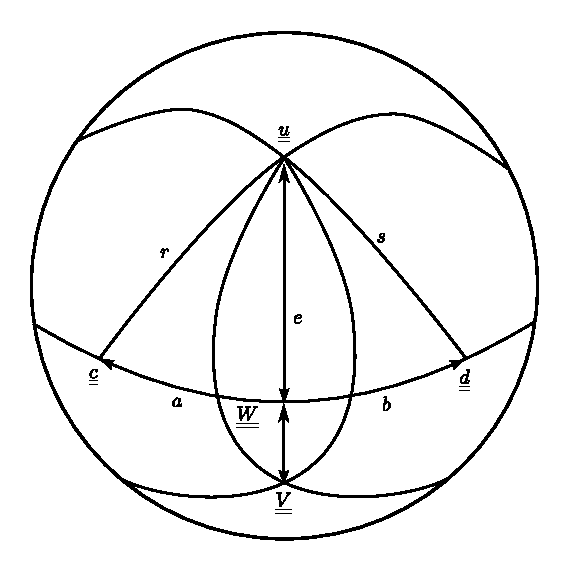
\includegraphics{fig3.eps}
\end{figure}

Let\pageoriginale $\uub{c}, \uub{d}$ be points with $\omega (\uub{c}, \uub{d}) = \omega$. The boundaries of $C(r, \uub{c})$ and $C(s, \uub{d})$ will intersect in two points $\uub{u}$ and $\uub{v}$. The big circle through $\uub{u}, \uub{v}$ will intersect the big circle through $\uub{c}, \uub{d}$ in two antipodal points $\uub{w}, \uub{w}'$. Of these two points, let $\uub{w}$ be the one with $\omega (\uub{w}, \uub{d}) = \omega$. Put
\begin{align*}
\omega (\uub{w}, \uub{u}) & = \omega (\uub{w}, \uub{v}) = e,\\
\omega (\uub{w}, \uub{c}) & = a, (\uub{w}, \uub{d}) = b
\end{align*}

Then
$$
a+b = \omega,
$$
and using the right spherical triangles $\uub{w}, \uub{u}, \uub{c}$ and $\uub{w}, \uub{u}, \uub{d}$ we obtain
$$
\cos a \cos e = \cos r, \cos b \cos e = \cos s.
$$


Combining these relations with the identities
$$
\cos x + \cos y = 2 \cos \frac{x+y}{2} \cos \frac{x-y}{2}
$$
and
$$
\cos x - \cos y = -2 \sin \frac{x+y}{2} \sin \frac{x-y}{2},
$$
we get
\begin{align*}
& \cos \frac{a+b}{2} \cos \frac{a-b}{2} \cos e = \cos \frac{r+s}{2} \cos \frac{r-s}{2},\\
& \sin \frac{a+b}{2} \sin \frac{a-b}{2} \cos e = \sin \frac{r+s}{2} \sin \frac{r-s}{2}.\\
\end{align*}

We now multiply the first of these two equations by $\sin \dfrac{\omega}{2}$, the second by $\cos \dfrac{\omega}{2}$, then square both and add. Since $\omega = a+b$, we obtain
\begin{align*}
& \sin^{2} \frac{\omega}{2} \cos^{2} \frac{\omega}{2} \cos^{2} e\\
& = \sin^{2} \frac{\omega}{2} \cos^{2} \frac{r+s}{2} \cos^{2} \frac{r-s}{2} + \cos^{2} \frac{\omega}{2} \sin^{2} \frac{r+s}{2} \sin^{2} \frac{r-s}{2}.
\end{align*}
which gives
\begin{equation*}
\sin^{2} e = \left(\sin^{2} \frac{\omega}{2} - \sin^{2} \frac{r-s}{2}\right) \left(\sin^{2} \frac{r+s}{2} - \sin^{2} \frac{\omega}{2}\right)^{-2} \left(\cos \frac{\omega}{2}\right)^{-2}.\tag{11.4}\label{chap2:sec11:eq11.4}
\end{equation*}\pageoriginale

We have seen that for $k = 2$, the boundaries of $C(r, \uub{c})$, $C(s, \uub{d})$ intersect two points $\uub{u}, \uub{v}$, and we defined numbers $a, b, e$ in terms of $\omega, r, s$. In general, we may assume a rotation that $\uub{c}, \uub{d}$ lie on the $x_{1}, x_{2}$- plane. Construct $\uub{w}$ so that $\omega (\uub{c}, \uub{w}) = a$, $\omega(\uub{d}, \uub{w}) = b$ ;  then $\uub{w}$ also lies in the $(x_{1}, x_{2})$- plane. By a further rotation, we may assume that $\uub{w} = (1, 0, \ldots, 0)$. Now let $\uub{z}$  be an arbitrary point on the intersection of the boundaries of $C(r, \uub{c}), C(s, \uub{d})$. There exists a rotation $\rho$ leaving points on the $(x_{1}, x_{2})$ - plane invariant such that $\rho (\uub{z})$ lies in the $(x_{1}, x_{2}, x_{3})$ - coordinate subspace. Then $\rho (\uub{z})$ again lies in the intersection of the boundaries of the two spherical caps, and therefore $\rho(\uub{z}) = \uub{u}$ or $\uub{v}$. Thus
$$
\rho (\uub{z}) = (\cos e, 0, \pm \sin e, 0, \ldots, 0),
$$    
and $\uub{z}$ itself is
$$
\uub{z} = (\cos e, 0, y_{3} \sin e, \ldots, y_{k+1} \sin e),
$$
where
$$
y_{3}^{2} + \ldots + y_{k+1}^{2} = 1.
$$

It follows that the intersection of the boundaries of the spherical caps $C(r, \uub{c})$, $C(s, \uub{d})$ consists of the points on the hyperplane $x_{2} = 0$ whose spherical distance from $\uub{w}$ is $e$.

The intersection $C(r, \uub{c}) \cap C(s, \uub{d})$ itself is contained in the set $W(e)$ of points whose spherical distance from the circle $x_{1}^{2} + x_{2}^{2} = 1$, $x_{2} = \ldots x_{k+1} = 0$ is $\leq e$. Put differently, $W(e)$ consists of points $(y_{1} \cos \varphi, y_{2}$ $\cos \varphi$, $y_{3} \sin \varphi, \ldots, y_{k+1} \sin \varphi$) with $y_{1}^{2} + y_{2}^{2} = 1$, $y_{3}^{2} + \ldots + y_{k+1}^{2} = 1$ and $0 \leq \varphi \leq e$. We note\pageoriginale that
$$
\mu(w(e)) = c_{1} \int_{0}^{e} \cos \varphi |\sin \varphi|^{k-2} d\varphi = c_{2} (\sin e)^{k-1}.
$$

Still under the assumption that $|r-s| < \omega < r+s$ , a simple geometric argument shows that as $\omega' \to \omega$,
$$
K(r, s, \omega) = K(r, s ; \omega') = \frac{(\omega' - \omega)}{2\pi} \mu (W(e)) + o(\omega - \omega').\footnote{The notation $f(t) = o(t)$ means that $f(t)/t$ tends to zero as $t > 0$ tends to zero.}
$$

This implies that
$$
\frac{\partial}{\partial \omega} (K(r, s ; \omega)) = -\frac{1}{2\pi} \mu (w(e)) = -c_{3} (\sin e)^{k-1}.
$$

In general we have
\begin{equation*}
\frac{\partial}{\partial \omega} (K(r, s ; \omega)) = 
\begin{cases}
-c_{3} (\sin e)^{k-1}, & \text{ if } |r - s| < \omega < r+s,\\
0, & \text{ otherwise. }
\end{cases}
\end{equation*}

The derivative of the left hand side of the integral equation (\ref{chap2:sec11:eq11.3}) with respect to $\omega$ is
\begin{align*}
& c_{3} \int_{\omega/2\delta}^{\frac{1}{2}} (\sin e(\delta r,\delta r, \omega))^{k-1} f(r) dr\\
& = -c_{3} \delta^{-1} \int_{\omega/2}^{\delta/2} f(r/\delta) (\sin e(r, r, \omega))^{k-1} dr.
\end{align*}

In view of (\ref{chap2:sec11:eq11.4}), this integral is equal to
\begin{equation*}
-c_{3} \delta^{-1} (\cos \omega)^{1-k} \int_{\omega/2}^{\delta/2} f(r/\delta) (\sin^{2} r - \sin^{2} \frac{\omega}{2})^{(k-1)/2} dr.\tag{11.5}\label{chap2:sec11:eq11.5}
\end{equation*}

Put $\Omega = \sin \dfrac{\omega}{2}/ \sin \dfrac{\delta}{2}$, $R = \sin r/2 \sin \dfrac{\delta}{2}$ and
$$
F(R) = f(r/\delta) \cos r.
$$

Now\pageoriginale if $\omega$ is in $0 \leq \omega \leq \delta$, then $\Omega$ is in $0 \leq \Omega \leq 1$, and if $0 \leq r \leq \delta/2$, then $0 \leq R \leq 1/2$. With these substitutions, (\ref{chap2:sec11:eq11.5}) becomes
\begin{equation*}
-c_{4} \delta^{-1} (\sin \frac{\delta}{2})^{k} (\cos \frac{\omega}{2})^{1-k} \int_{\Omega/2}^{\frac{1}{2}} F(R)(R^{2} - \frac{\Omega^{2}}{4})^{(k-1)/2} dR.
\end{equation*}

The right hand side of the integral equation after differentiation with respect to $\omega$ becomes
\begin{multline*}
-c_{5} \delta^{\nu-1} \mathop{\int_{0}^{\delta} \int_{0}^{\delta}}_{|r-s|\leq \omega \leq r+s \leq \delta} (\sin e(r, s, \omega))^{k-1} \cos \frac{r-s}{2} \cos \frac{r+s}{2}\\ 
\left(\sin \frac{|r-s|}{2}\right)^{-\alpha} \left(\sin \frac{r+s}{2}\right)^{-\beta} dr ~ ds.
\end{multline*}

Substituting the value of $\sin e$ as given by $(11.4)$, we obtain
\begin{multline*}
-c_{5} \delta^{\nu-1} \left(\sin \frac{\omega}{2}\right)^{-(k-1)} \left(\cos \frac{\omega}{2}\right)^{-(k-1)} \times \\
\mathop{\int_{0}^{\delta} \int_{0}^{\delta}}_{|r-s|\leq \omega \leq r+s \leq \delta} \left(\sin^{2} \frac{\omega}{2} - \sin^{2} \frac{r-s}{2}\right)^{(k-1)/2} \left(\sin^{2} \frac{r+s}{2} - \sin^{2} \frac{\omega}{2}\right)^{\left(\frac{k-1}{2}\right)} \times\\
\cos \frac{r-s}{2} \cos \frac{r+s}{2} \left(\sin \frac{|r-s|}{2}\right)^{-\alpha} \left(\sin \frac{r+s}{2}\right)^{-\beta}dr~ds.
\end{multline*}

Put
$$
\Omega = \sin \frac{\omega}{2} / \sin \frac{\delta}{2}, x = \sin \frac{r+s}{2}/\sin \frac{\delta}{2}, y = \sin \frac{|r-s|}{2}/\sin \frac{\delta}{2}.
$$

The above integral then becomes
\begin{multline*}
-c_{6} \delta^{\nu - 1} (\sin \frac{\delta}{2})^{k-\alpha-\beta+1} (\cos \frac{\omega}{2})^{1-k} \times\\
\int_{\Omega}^{1} (x^{2} - \Omega^{2})^{(k-1)/2} x^{-\beta} dx \int_{0}^{\Omega} (1 - \frac{y^{2}}{\Omega^{2}})^{(k-1)/2} y^{-\alpha} dy\\
= -c_{7} \delta^{\nu - 1} (\sin \frac{\delta}{2})^{k-\nu} (\cos \frac{\omega}{2})^{1-k} \Omega^{1-\alpha} \int_{\Omega}^{1} (x^{2} - \Omega^{2})^{(k-1)/2} x^{-\beta} dx.
\end{multline*}

Hence we obtain the new integral equation
\begin{align*}
& \int_{\Omega/2}^{\frac{1}{2}} F(R) (R^{2} - \frac{\Omega^{2}}{4})^{(k-1)/2} dR\\
& = c_{8} \left(\frac{\delta}{\sin \frac{\delta}{2}}\right)^\gamma \Omega^{1-\alpha} \int_{\Omega}^{1} (x^{2} - \Omega^{2})^{(k-1)/2} x^{-\beta} dx \quad (0 < \Omega < 1).\tag{11.6}\label{chap2:sec11:eq11.6}
\end{align*}\pageoriginale

\label{105}
If $F(R)$ is a solution of this integral equation, then $f(r) = F(r
\delta)\break\cos r \delta$ is a solution of the given integral equation
(\ref{chap2:sec11:eq11.3}). 

Except for the factor $(\delta /\sin (\delta/2))^\nu$ and except for the notation, this integral equation is the same as (\ref{chap2:sec3:eq3.6}). Hence there is a solution of (\ref{chap2:sec11:eq11.6}) of the type
$$
F(R) = F_{0}(R) - F_{*} (R),
$$
where $F_{0}(R)$ and $F_{*}(R)$ are positive and continuous in $0 < R \leq 1/2$, and have
\begin{equation*}
F_{0} (R) \gg \ll R^{1 - \nu - \alpha} \text{ and } F_{*}(R) \gg \ll R^{1-k-\alpha},\tag{11.7}\label{chap2:sec11:eq11.7}
\end{equation*}
as $R \to 0$. These functions depend on $\delta$; they are $(\delta /\sin (\delta/2))^{\nu}$ times functions which are independent of $\delta$. Since
$$
\delta / \sin (\delta/2) \gg \ll 1,\qquad (0 < \delta <\pi/2)
$$
the estimates (\ref{chap2:sec11:eq11.7}) hold uniformly in $\delta$.

By what we said above the function
$$
f(r) = f_{0}(r) - f_{*}(r)
$$
with $f_{0} (r) = F_{0} (\delta r) \cos \delta r$, $f_{*}(r) = F_{*}(\delta r) \cos \delta r$, is a solution of the original equation (\ref{chap2:sec11:eq11.3}). The functions $f_{0}(r)$ and $f_{*}(r)$ are positive and continuous in $0 < r \leq 1/2$, and $r \to 0$ they satisfy
$$
f_{0} (r) \gg \ll r^{1-\nu - \alpha} \text{ and } f_{*}(r) \gg \ll r^{1-k-\alpha},
$$
uniformly in $\delta$.

In\pageoriginale view of the Fundamental Lemma and by the definition of $A$,
\begin{equation*}
\int_{0}^{\frac{1}{2}} E(\delta r, \delta r) f(r) dr = A.
\end{equation*}
and 
\begin{equation*}
\int_{0}^{\frac{1}{2}} E(\delta r, \delta r) f_{0} (r) dr - A = \int_{0}^{\frac{1}{2}} E(\delta r, \delta r) f_{*} (r) dr.\tag{11.8}\label{chap2:sec11:eq11.8}
\end{equation*}

In view of (\ref{chap2:sec11:eq11.1}) and since $f_{0}(r) \ll r^{1 - \nu - \alpha} \ll r^{-1}$, the left hand side of this equation is
$$
\ll \int_{0}^{\delta} E(r, r) r^{-1} dr.
$$

On the other hand $|D(r, \uub{c})| \geq ||N\mu(s)||$, whence $E(r, r) \geq ||N\mu(r)||^{2}$, and the right hand side of (\ref{chap2:sec11:eq11.8}) is
$$
\gg \int_{0}^{c_{9}} r^{1-k-\alpha} E(\delta r, \delta r) dr \geq \int_{0}^{c_{9}} r^{1-k-\alpha} ||N\mu(\delta r)||^{2} dr.
$$

A suitable adaptation of the argument below (\ref{chap2:sec4:eq4.5}) shows that this is $\gg (N \delta^{k})^{1 + (\alpha/k)-(2/k)}$, and hence also
$$
\int_{0}^{\delta} E(r, r) r^{-1} dr \gg (N \delta^{k})^{1+(\alpha/k)-(2/k)}.
$$

Since $\alpha$ was arbitrary in $0 < \alpha < 1$, Theorem $10A$ is proved.

\section{Point with Weights}\label{chap2:sec12} 

Many results of these lectures may be generalized to distributions of points with weights. As a sample, we will now mention a partial generalization of Theorem 10\ref{chap2:sec10:thm10A}.

Let $\uub{p}_{1}, \ldots, \uub{p}_{N}$ be points on the sphere $S = S^{k}$. Suppose that non-negative weights $w_{1}, \ldots, w_{N}$ are attached to these points. Now given a measurable subset $A$ of $S$, write
\begin{align*}
z(A) & = \sum_{\uub{p}_{i} \in A} w_{i},\\
D(A) & = z(A) -\mu(A) z(S).
\end{align*}

\begin{theorem}[$^*$. (W. M. Schmidt \cite{23})]\label{chap2:sec12:thm12A}
Suppose\pageoriginale that $\in > 0$. There exists a spherical cap $C(r, \uub{c})$ with
$$
|D(C(r, \uub{c}))| \gg (w_{1}^{2} + \ldots + w_{N}^{2})^{1/2} N^{-(1/2k)- \epsilon} .
$$
\end{theorem}

Results about countable distributions of points with a finite total weight may also be obtained.

\section{Convex Sets}\label{chap2:sec13}

\begin{theorem}[(W. M. Schmidt \cite{27})]\label{chap2:sec13:thm13A} 
Suppose $0 < \delta < 1$. There exists a convex set $S$ in $U^{k}$ with diameter $\leq \delta$ and with 
$$
|D(S)| \gg (N \delta^{k})^{1-(2/(k+1))}.
$$
\end{theorem}

This is stronger than an earliest estimate due to S. K. Zaremba \cite{30}.

By a {\em quadrant set} we shall understand a subset $Q$ of $U^{k}$ with the property that if $\uub{y} = (y_{1}, \ldots, y_{k}) \in Q$, then the box consisting of $\uub{x} = (x_{1}, \ldots, x_{k})$ with $0 \leq x_{i} \leq y_{i} (i = 1, \ldots, k)$ is contained in $Q$.

\begin{theorem}\label{chap2:sec13:thm13B}
Suppose $0 < \delta < 1$. There is a quadrant set $Q$ of diameter $\leq \delta$ with
$$
|D(Q)| \gg (N \delta^{k})^{1-(1/k)}
$$
\end{theorem}

\medskip
\noindent{\textit{Proof of Theorem 13\ref{chap2:sec13:thm13A}.}} We may suppose that $k > 1$, and that $N \delta^{k}$ is large. Let $B$ be a ball of diameter $\delta$ contained in $U^{k}$, and let $S$ be the surface of $B$. Let $C$ be a closed spherical cap on $S$ with spherical radius $\rho$. (With the radius normalized such that a half sphere has radius $\frac{\pi}{2}$). The convex hull $\overline{C}$ of $C$ is a solid spherical cap. For $0 < \rho < \frac{\pi}{2}$, $\mu(\overline{C})$ is a continuous function of $\rho$ with
\begin{equation*}
\rho^{k+1} \delta^{k} \ll \mu(\overline{C}) \ll \rho^{k+1} \delta^{k}.\tag{13.1}\label{chap2:sec13:eq13.1}
\end{equation*}\pageoriginale

If $N \delta^{k}$ is sufficiently large, there is a number $\rho_{0}$ such that a cap $C$ of spherical radius $\rho_{0}$ has
$$
\mu(C) = \frac{1}{2N}.
$$

In view of (\ref{chap2:sec13:eq13.1}), $0 < \rho_{0} \ll (N \delta^{k})^{-1/(k+1)}$. We now pick as many pairwise disjoint caps with radius $\rho_{0}$ as possible; say $C_{1}, \ldots, C_{M}$. For large $N \delta^{k}$ and hence small $\rho_{0}$ we have $M \gg \rho_{0}^{-(k-1)}$, whence
\begin{equation*}
M \gg (N \delta^{k})^{(k-1)/(k+1)}.\tag{13.2}\label{chap2:sec13:eq13.2}
\end{equation*}

Given a sequence of numbers $\sigma_{1}, \ldots, \sigma_{M}$, with each $\sigma_{i}$ either $+1$ or $-1$, let $B(\sigma_{1}, \ldots, \sigma_{M})$ consist of all $\uub{x} \in B$ which do not lie in a cap $\overline{C}_{i}$ with $\sigma_{i} = -1$. In other words, $B(\sigma_{1}, \ldots, \sigma_{M})$ is obtained from $B$ by removing the solid caps $\overline{C}_{i}$ for which $\sigma_{i} = -1$.

Now the function $D(A)$ is {\em additive}, i. e. it satisfies
$$
D(A \cup A') = D(A) + D(A')
$$
if $A \cap A' = \phi$. It follows easily that
$$
D(B(\sigma_{1}, \ldots, \sigma_{M})) - D(B(-\sigma_{1}, \ldots, -\sigma_{M})) = \sum_{i=1}^{M} \sigma_{i} D(\overline{C}_{i}).
$$

We have
$$
D(\overline{C}_{i}) = z(\overline{C}_{i}) - N\mu(\overline(C)_{i}) = z(\overline{C}_{i}) - \frac{1}{2}.
$$

Hence for every $i$, either $D(\overline{C}_{i}) \geq \frac{1}{2}$ or $D(\overline{C}_{i}) \leq - \frac{1}{2}$. Choose $\sigma_{i}$ such that $\sigma_{i} D(\overline{C}_{i}) \geq \frac{1}{2} (1 \leq i \leq M)$. Then
$$
D(B(\sigma_{1}, \ldots, \sigma_{M})) -D(B(-\sigma_{1}, \ldots, -\sigma_{M})) \geq \frac{1}{2} M,
$$
and\pageoriginale either $S = B(\sigma_{1}, \ldots, \sigma_{M})$ or $S = B(-\sigma_{1}, \ldots, -\sigma_{M})$ has $|D(S)| \geq \frac{1}{2} M$. Thus by $(13.2)$,
$$
|D(S)| \gg (N \delta^{k})^{(k-1)/(k+1)}.
$$

Theorem 13\ref{chap2:sec13:thm13A} is proven.

\medskip
\noindent{\textit{Proof of Theorem 13\ref{chap2:sec13:thm13B}.}} We may suppose that $k > 1$, and that $N \delta^{k}$ is large. Let $G$ consist of points in $U^{k}$ with $x_{1} + \ldots, +x_{k} \leq \delta/k$, and $H$ of points with $x_{1} + \ldots + x_{k} = \delta/k$. Let $\in > 0$ be small, and let $\uub{x} = (x_{1}, \ldots, x_{k})$ be a points on $H$ with $(k-1) \delta \in < x_{i} (i=1, \ldots, k)$. Let $P(\uub{x})$ consist of points $\uub{y} = (y_{1}, \ldots, y_{k})$ with
$$
y_{1} + \ldots +y_{k} . >\delta/k \text{ and } y_{i} \leq x_{i} + \delta \in (i = 1, \ldots, k).
$$

Then $P(\uub{x})$ lies in $U^{k}$ and has volume $\mu (P(\uub{x})) =
(k \delta \epsilon)^{k}/k!$. If $N \delta^{k}$ is sufficiently large,
we may choose $\epsilon$ such that this volume equals $1/(2N)$. Then
$\epsilon \ll (N \delta^{k})^{-1/k}$. 

Pick as many pairwise disjoint sets $P(\uub{x})$ as possible ; say
$P_{1}, \ldots, P_{M}$. Clearly $M \gg \in^{-(k-1)}$, whence 
$$
M \gg (n \delta^{k})^{(k-1)/k}.
$$

For any sequence $\sigma_{1}, \ldots, \sigma_{M}$ of $+1$ and $-1$ signs, let $Q(\sigma_{1}, \ldots, \sigma_{M})$ be the union of $G$ with the ``blisters'' $P_{i}$ for which $\sigma_{i} = 1$. Th set $Q(\sigma_{1}, \ldots, \sigma_{M})$ is a quadrant set of diameter $\leq \delta$. We have
$$
D(Q(\sigma_{1}, \ldots, \sigma_{M})) - D(Q(-\sigma_{1}, \ldots, -\sigma_{M})) = \sum_{i=1}^{M} \sigma_{i} D(Q_{i}).
$$

By an argument used in the proof of Theorem 13\ref{chap2:sec13:thm13A}, we obtain a quadrant set $Q$ of diameter $\leq \delta$ with
$$
|D(Q)| \geq \frac{1}{4} M \gg (N \delta^{k})^{(k-1)/k}.
$$

\section{Comparison of different discrepancies}\label{chap2:sec14}

If\pageoriginale $\mathfrak{a}$ is anon-empty class of measurable sets in $U^{k}$, write
$$
D(\mathfrak{a}) = \sup |D(A)|,
$$
where the supermum is over all $A \in \mathfrak{a}$. Further put
$$
\triangle (\mathfrak{a}) = D(\mathfrak{a})/N.
$$

It is clear that $0 \leq D(\mathfrak{a}) \leq N$ and $o \leq \triangle (\mathfrak{a}) \leq 1$. One could call $D(\mathfrak{a})$ the {\em discrepancy with respect to} $\mathfrak{a}$ of the given $N$ points; but some authors prefer to call $\triangle (\mathfrak{a})$ the discrepancy.

Let $\mathscr{J}$ be the class of boxes in $U^{k}$ of the type $a_{1} \leq x_{1} \leq b_{1}, \ldots, a_{k}$ $\leq x_{k} \leq b_{k}$, let $\mathfrak{M}$ be the class of closed cubes in $U^{k}$ with sides parallel to the coordinate axes, $\mathscr{L}$ the class of closed balls in $U^{k}$, $\mathfrak{S}$ the class of convex subsets of $U^{k}$ and $\mathfrak{q}$ the class of quadrant sets.

We have already seen that
\begin{align*}
& \triangle(\mathfrak{J}) \gg N^{-1}(\log N)^{(k-1)/2}  & \text{(Ch. I, Theorem 2\ref{chap1:sec2:thm2B})},\\
& \triangle(\mathfrak{J}) \gg N^{-1}(\log N) \text{ if } k = 2  & \text{(Ch. I, Theorem 5\ref{chap1:sec5:thm5B})},\\
& \triangle{\mathscr{L}} \gg N^{(k-1)/(2k(k+2))-1-\epsilon} & \text{(Corollary to Theorem 6\ref{chap2:sec6:thm6A})}\\
& \triangle{\mathfrak{S}} \gg N^{-2/(k+1)} & \text{(Theorem 13\ref{chap2:sec13:thm13A})}
\end{align*}
and that
$$
\triangle(\mathfrak{q}) \gg N^{-1/k} \qquad (\text{Theorem 13\ref{chap2:sec13:thm13B}}).
$$

Now $\mathfrak{a} \leq \mathfrak{a}'$ implies $\triangle(\mathfrak{a}) \leq \triangle(\mathfrak{a}')$, so that
\begin{align*}
\triangle(\mathfrak{M}) \leq \triangle(\mathfrak{J}) \leq \triangle (\mathfrak{S}),\\
\triangle (\mathscr{L}) \leq \triangle (\mathfrak{S}).
\end{align*}

\begin{theorem}[ (W. M. Schmidt \cite{27})]\label{chap2:sec14:thm14A}
\begin{align*}
\triangle (\mathfrak{S}) & \ll \triangle(\mathfrak{M})^{1/k}\\
\triangle (\mathfrak{q}) & \ll \triangle(\mathfrak{M})^{1/k}\\.
\end{align*}\pageoriginale
\end{theorem}

Earlier, E. Hlawka \cite{10} (see also \cite{9}) had shown that $\triangle(\mathfrak{S})$\break $\ll \triangle(\mathfrak{m})^{1/(k+1)}$ and $\triangle(\mathfrak{S}) \ll \triangle (\mathfrak{J})^{1/k}$.

Write exp $x = e^{x}$.

\begin{theorem}\label{chap2:sec14:thm14B}
Both $\triangle(\mathfrak{S})$ and $\triangle(\mathfrak{q})$ are
$$
\ll \triangle(\mathscr{L})^{1/k} exp (2(\log 2)^{1/2} k^{-1} |\log \triangle (\mathscr{L})|^{1/2}).
$$
\end{theorem}

In particular, it follows that for $\in > 0$, both $\triangle (\mathfrak{S})$ and $\triangle (\mathfrak{q})$ are
$$
\ll \triangle (\mathscr{L})^{(1/k)-\epsilon}.
$$

This is stronger than estimates of Hlawka \cite{10}. J. W. S. Cassels (unpublished) and C. J. Smyth \cite{28}. But on the other hand Smyth (thesis, Cambridge, Engaland) obtained
$$
\triangle(\mathfrak{J}) \ll \triangle(\mathscr{L})^{1/k} (1 + \log |\triangle (\mathscr{L})|^{c(k)}).
$$
which will not be proved here.

Let $B(r, \uub{c})$ be the closed ball with radius $r$ and center $ \uub{c}$. Given a subset $S$ of $U^{k}$, let $S(r)$ consist of points $ \uub{x}$ for which $B(r,  \uub{x}) \subseteq S$. Let $S'$ be the complement of $S$ in $U^{k}$.

For each $\sigma > 0$. let $\mathfrak{S} (\sigma)$ be the class of subsets $S$ of $U^{k}$ having 
\begin{equation*}
\mu (S(r)) \geq \mu(S) - \sigma r, \mu (S'(r)) \geq \mu(S') - \sigma r\tag{14.1}\label{chap2:sec14:eq14.1}
\end{equation*}
for every $r > 0$.

\begin{lemma}\label{chap2:sec14:lem14C}
There are constants $c_{1}(k)$, $c_{2}(k)$ such that
$$
\mathfrak{S} \subseteq \mathfrak{S} (c_{1}). \mathfrak{q} \subseteq (c_{2}).
$$
\end{lemma}

The\pageoriginale proof of this lemma is easy and will not be given here. For a rather more thorough discussion of $\mu(S(r))$ for convex sets $S$, see H. G. Eggleston \cite{4}.

Theorem 14\ref{chap2:sec14:thm14A}, 14\ref{chap2:sec14:thm14B} are respective consequences of

\setcounter{theorem}{2}
\begin{theorem}\label{chap2:sec14:thm14C}
$$
\triangle (\mathfrak{S}(\sigma)) \leq c_{3} (k, \sigma) \triangle (\mathfrak{M})^{1/k}
$$
\end{theorem} 

\begin{theorem}\label{chap2:sec14:thm14D} 
$$
\triangle(\mathfrak{S} (\sigma)) \leq c_{4} (k, \sigma) \triangle(\mathscr{L})^{1/k} exp (2(\log 2)^{1/2} k^{-1} |\log \triangle (\mathscr{L})|^{1/2}).
$$
\end{theorem}

\medskip
\noindent \textit{Proof of Theorem 14\ref{chap2:sec14:thm14C}}. Let $S[r]$ consist of points $\uub{x} \in U^{k}$ which have a distance $< r$ from the boundary of $S$. Every $\uub{x} \in S[r]$ is either in $S$ but not in $S(r)$, or is in $S'$ but not in $S'(r)$. Hence for $S \in \mathfrak{S}(\sigma)$.
$$
\mu (S[r]) \leq 2 \sigma r.
$$

Now if $k = 1$ and if $z_{1}, \ldots, z_{M}$ are on the boundary of $S$ and in the interior of $U$, then for small $r$, $S[r]$ contains the $M$ open intervals with centres $z_{1}, \ldots, z_{M}$ and of length $2r$. Hence for small $r, \mu(S[r]) \geq 2r M$, and we get $M \leq \sigma$. Thus $S$ has at most $\sigma + 2$ boundary points, and is therefore the union of a bounded numbers of points and intervals. Hence Theorem 14\ref{chap2:sec14:thm14C} is true for $k = 1$.

We may henceforth assume that $k > 1$. Pick a point $\uub{a} = (a_{1}, \ldots, a_{k})$ such that for each of the given points $\uub{p}_{i} (i = 1, \ldots, N)$, each coordinate of $\uub{p}_{i} - \uub{a}$ irrational. For a positive integer $n$, let $\mathfrak{M} (n)$ be the class of cubes
$$
a_{i} + \frac{u_{i}}{n} \leq x_{i} \leq a_{i} + \frac{u_{i} + 1}{n} (i = 1, \ldots, k)
$$
with integers $u_{1}, \ldots, u_{k}$. Let $\mathfrak{W} (n)$ be the set of cubes of $\mathfrak{M} (n)$ which are contained in $S$. Since a cube of $\mathfrak{M} (n)$ has diameter $k^{\frac{1}{2}}/n$, it follows that the cubes of $\mathfrak{W} (n)$ cover $S(k^{\frac{1}{2}}/n)$, and their number $\nu(n)$ satisfies
\begin{equation*}
n^{k} \mu(S) \geq \nu(n) \geq n^{k} \mu (S(k^{\frac{1}{2}}/n)) \geq n^{k} \mu (S) - n^{k-1} \sigma k^{\frac{1}{2}}.\tag{14.2}\label{chap2:sec14:eq14.2}
\end{equation*}\pageoriginale

For each positive integer $i$, the union of the cubes of $\mathfrak{W}(2^{i})$ contains the union of the cubes of $\mathfrak{W} (2^{i-1})$. Put $\mathfrak{W}_{1}= \mathfrak{W} (2^{1})$, and for $i \geq 2$. let $\mathfrak{W} i$ consist of the cubes of $\mathfrak{W} (2^{i})$ which are not contained in a cube of $\mathfrak{W} (2^{i-1})$. If $\nu_{i}$ is the number of cubes in $\mathfrak{W}_{i}$, then $\nu_{1} = \nu(2)$, and for $i \geq 2$ we have
$$
2^{-ik} \nu_{i} + 2^{-(i - 1)k} \nu(2^{i-1}) \leq \mu(S),
$$
whence by (\ref{chap2:sec14:eq14.2}),
$$
\nu_{i} \leq 2^{ik} \nu(S) - 2^{k} \nu (2^{i-1}) \leq \sigma k^{\frac{1}{2}} 2^{i(k-1)+1}.
$$

Since any two distinct cubes in any of the sets $\mathfrak{W}_{1}, \mathfrak{W}_{2}, \ldots$ are disjoint except possibly for their boundaries, and since by our choice of $\uub{a}$ none of the given $N$ points lie on such a boundary, we have for every positive integer $M$,
\begin{align*}
z(S) & \geq \sum_{i=1}^{M} \sum_{W \epsilon \mathfrak{W}_{i}} z(W)\\
\geq & \sum_{i=1}^{M} \sum_{W \epsilon \mathfrak{W}_{i}} (N \mu (W) - N \triangle (\mathfrak{M}))\\
= & N\left(\left(\sum_{W \epsilon \mathfrak{W} (2^{M})}\right) \mu(W)) - \triangle (\mathfrak{M}) \sum_{i=1}^{M} \nu_{i}\right)\\
\geq & N\left(\mu \left(S\left(k^{\frac{1}{2}} 2^{-M}\right)\right) - \triangle (\mathfrak{M}) \left(2^{k} + \sigma k^{\frac{1}{2}} \sum_{i=2}^{M} 2^{i(k-1)+1}\right)\right)\\
\geq & N \mu (S) - N c_{5} (k, \sigma) (2^{-M} + \triangle (\mathfrak{M}) 2^{M(k-1)}),\\
\end{align*}
since $k > 1$. Now if we choose $M$ such that $2^{M-1} \leq \triangle (\mathfrak{M})^{-1/k} < 2^{M}$, then 
$$
z(S) - N\mu(S) \geq - Nc_{5}(k, \sigma) \triangle (\mathfrak{M})^{1/k} (1+2^{k-1}) = -N c_{3}(k, \sigma) \triangle (\mathfrak{M})^{1/k}.
$$

This inequality remains true if we replace $S$ by $S'$. Hence
$$
|z(S) - N\mu(S)| \leq N c_{3} (k, \sigma) \triangle (\mathfrak{W})^{1/k},
$$ 
and\pageoriginale Theorem 14\ref{chap2:sec14:thm14C} follows.

\section{Proof of Theorem 14\ref{chap2:sec14:thm14D} by ``successive sweeping''} \label{chap2:sec15}

Given a set $A$,let $rA + \uub{y}$ be the set of points $r\uub{a} + \uub{y}$ with $\uub{a} \in A$. Let $\mathfrak{a}(A)$ be the class of sets $rA + \uub{y}$ with $r > 0$ which are contained in $U^{k}$. Thus if $B$ is any closed ball, then $\mathfrak{a}(B) = \mathscr{L}$. Hence Theorem 14\ref{chap2:sec14:thm14D} follows from
\begin{theorem}\label{chap2:sec15:thm15A}
Suppose $\mu(A) > 0$ and $A \in \mathfrak{S} (\tau)$ for some $\tau$. Then 
$$
\triangle(\mathfrak{S} (\sigma)) \leq c_{1} (A, \sigma) 
\triangle(\mathfrak{a}(A))^{1/k} exp (2(\log 2)^{\frac{1}{2}} k^{-1} |\log \triangle (\mathfrak{a}(A))|^{\frac{1}{2}}).
$$
\end{theorem}
 
The proof of this theorem will require a series of lemmas. Denote the distance of points $x$, $y$ by
$$
|\uub{x} - \uub{y}|.
$$

Now let $r_{1}, r_{2}, \ldots$ be positive reals with
\begin{equation*}
r_{i+1} \leq \frac{1}{2} r_{i} \quad{i = 1, 2, \ldots}.\tag{15.1}\label{chap2:sec15:eq15.1}
\end{equation*}
and set $s_{i} = k^{\frac{1}{2}} r_{i}$. The set $r_{i} A$ has diameter $\leq s_{i}$.

For a set $T$, let $\mathcal{X} (T | \uub{x})$ be the characteristic function of $T$. Let $S$ be a set belonging to $\mathfrak{S}(\sigma)$.

We are going to construct functions $f_{\nu} (\uub{x})$, $g_{\nu} (\uub{x})$, $h_{\nu} (\uub{x})$ $(\nu = 0, 1, 2$, $\ldots)$.

We begin by setting
$$
f_{0}(\uub{x}) = 0.
$$

If a continuous function $f_{\nu} (\uub{x})$ is given, write
\begin{align*}
g_{\nu} (\uub{x}) & = \mathcal{X}(S | \uub{x}) - f_{\nu} (\uub{x}),\\
h_{\nu} (\uub{x}) & = \min_{|\uub{y} - \uub{x}| \leq s_{\nu+1}} g_{\nu} (\uub{y}),\\
f_{\nu+1} (\uub{x}) &= f_{\nu} (\uub{x}) + (\nu(r_{\nu+1} A))^{-1} \int \mathcal{X} (r_{\nu+1} A + \uub{y} | \uub{x}) h_{\nu} (\uub{y}) d\uub{y}.
\end{align*}

\begin{lemma}\label{chap2:sec15:lem15B}
We\pageoriginale have
\begin{enumerate}
\item[\rm(i)] $0 \leq f_{\nu-1} (\uub{x}) \leq f_{\nu} (\uub{x}) \leq \mathcal{X} (S | \uub{x}) \qquad (\nu = 1, 2, \ldots)$,
\item[\rm(iia)] $|f_{\nu}(\uub{x}) - f_{\nu}(\uub{x}')| \leq c_{2} (A) r_{\nu}^{-1} |\uub{x} - \uub{x}'| \qquad (\nu = 1, 2, \ldots)$,
 and in particular $f_{\nu}(\uub{x})$ is continuous.
\item[\rm(iib)] $|f_{\nu} (\uub{x}) - f_{\nu}(\uub{x}')| \leq 2^{\nu - i} c_{2} (A) r_{i}^{-1} |\uub{x} - \uub{x}'|$
if $i \leq i \leq \nu - 1$ and if $|\uub{x} - \uub{x}'| \leq s_{\nu}$ and $\uub{x}$, $\uub{x}' \in S(3(s_{i+1} + \ldots + s_{\nu})).$
\item[\rm(iiia)] $f_{\nu} (\uub{x}) = 1$ if $\uub{x} \in S(2s_{1}) \qquad (\nu = 1, 2, \ldots)$,
\item[\rm(iiib)] $f_{\nu} (\uub{x}) \geq 1 - 2^{\nu-i} c_{3} (A) (s_{\nu}/s_{i})$ if $1 \leq i \leq \nu - 1$ and $\uub{x} \in S(6s_{i+1})$.
\end{enumerate}
\end{lemma}

Our construction may be interpreted as follows. We first sweep $S$ with a broom of the size and shape of $r_{1}A$. We can sweep the middle of $S$, more precisely $S(2s_{1})$, very well. But we cannot sweep the border areas of $S$ very well. We then take a smaller broom of the size and shape of $r_{2} A$. And so on. We obtain a better and better sweeping of $S$ which is expressed by $(i)$ and $(iiib)$. But it would have been inefficient to sweep right away with a very small broom of the size and shape of $r_{\nu} A$.

\begin{proof} 
We proceed by induction on $\nu$. Assume that either $\nu = 0$ or that the lemma is true for a particular value of $\nu > 0$. We have $0 \leq f_{\nu} (\uub{x}) \leq \mathcal{X}(S | \uub{x})$, whence $0 \leq g_{\nu} (\uub{x}) \leq \mathcal{X}(S | \uub{x})$. Now if $\uub{y} \in r_{\nu+1} A + \uub{x}$, then $\uub{y} - \uub{x} \in r_{\nu+1} A$, whence $|\uub{y} - \uub{x}| \leq s_{\nu+1}$, whence $h_{\nu} (\uub{y}) \leq g_{\nu}(\uub{x})$. We obtain
\begin{align*}
0 \leq \int \mathcal{X} (r_{\nu+1} A + \uub{y}\backslash \uub{x}) h_{\nu} (\uub{y}) d\uub{y} & \leq g_{\nu}(\uub{x}) \int \mathcal{X} (r_{\nu+1} A + \uub{y}\backslash \uub{x}) d\uub{y}\\
& = g_{\nu} (\uub{x}) \mu(r_{\nu+1} A).
\end{align*}
and\pageoriginale
$$
f_{\nu} (\uub{x}) \leq f_{\nu+1} (\uub{x}) \leq f_{\nu} (\uub{x}) + g_{\nu} (\uub{x}) = \mathcal{X}(S \backslash \uub{x}).
$$
Hence $(i)$ is true for $\nu + 1$.
\end{proof}

Now it is clear that $\ell_{\nu+1} (\uub{x}) = f_{\nu+1}(\uub{x}) - f_{\nu}(\uub{x})$ has
\begin{multline*}
\ell_{\nu+1} (\uub{x}) - \ell_{\nu+1} (\uub{x}') = (\mu(r_{\nu+1} A))^{-1}\\ \int\left(\mathcal{X} (r_{\nu+1} A + \uub{y} \backslash \uub{x}) - \mathcal{X} (r_{\nu+1} A + \uub{y} \backslash \uub{x}')\right) h_{\nu} (\uub{y}) d\uub{y}.
\end{multline*}

Since $0 \leq h_{\nu} (\uub{y}) \leq 1$, we obtain
$$
\ell_{\nu+1} (\uub{x}) - \ell_{\nu+1} (\uub{x}') \leq (\mu(r_{\nu+1} A))^{-1} \mu(C_{1}),
$$
where $C_{1}$ consists of $\uub{y}$ for which $-\uub{y}$ lies in $r_{\nu+1} A - \uub{x}$ but not in $r_{\nu+1} A - \uub{x}'$. Now
$$
\mu(C_{1}) = r_{\nu+1}^{k} \mu(C_{2}),
$$
where $C_{2}$ consists of $\uub{y}$ which are in $A - r_{\nu+1}^{-1} (\uub{x} - \uub{x}')$ but not in $A$. Now if $\uub{y} \in C_{2}$ lies in $U^{k}$, then $\uub{y} \in A'$ and $\uub{y} \notin A'(r_{\nu+1}^{-1} |\uub{x} - \uub{x}'|)$. Hence by virtue of $A \in \mathfrak{S} (\tau)$, the intersection $C_{2} \cap U^{k}$ has volume $\leq \tau r_{\nu+1}^{-1} |\uub{x} - \uub{x}'|$. On the other hand if $\uub{y} \in C_{2}$ lies putside of $U^{k}$, then, it has distance $\leq r_{\nu+1}^{-1} |\uub{x} - \uub{x}'|$ from $U^{k}$, and if $r_{\nu+1}^{-1} |\uub{x} - \uub{x}'| \leq 1$, then the part of $C_{2}$ outside $U^{k}$ has volume $\leq 6^{k} r_{\nu+1}^{-1} |\uub{x} - \uub{x}'|$. Thus if $|\uub{x} - \uub{x}'|$ is small, then $\mu(C_{2}) \leq (\tau + 6^{k}) r_{\nu+1}^{-1} |\uub{x} - \uub{x}'|$, and therefore
$$
\ell_{\nu+1} (\uub{x}) - \ell_{\nu+1} (\uub{x}') \leq \frac{1}{2} c_{2} (A) r_{\nu+1}^{-1} |\uub{x} - \uub{x}'|.
$$
with $c_{2}(A) = 2\mu(A)^{-1} (\tau + 6^{k})$. It follows that for {\em every} $\uub{x}$, $\uub{x}'$,
\begin{equation*}
|\ell_{\nu+1} (\uub{x}) - \ell_{\nu+1} (\uub{x}')| \leq \frac{1}{2} c_{2} (A) r_{\nu+1}^{-1} |\uub{x} - \uub{x}'|.\tag{15.2}\label{chap2:sec15:eq15.2}
\end{equation*}

Now if $\nu = 0$, we have $f_{\nu+1}(\uub{x}) = f_{1}(\uub{x}) = \ell_{1} (\uub{x})$, and the case $\nu = 1$ of (iia) follows. If $\nu > 0$, we use our inductive assumption, (\ref{chap2:sec15:eq15.1}), (\ref{chap2:sec15:eq15.2}) and the relation $f_{\nu+1} (\uub{x}) = f_{\nu}(\uub{x}) + \ell_{\nu+1} (\uub{x})$ to obtain
$$
|f_{\nu+1} (\uub{x}) - f_{\nu+1} (\uub{x}')| \leq (c_{2}(A) r_{\nu}^{-1} + \frac{1}{2} c_{2} (A) r_{\nu+1}^{-1}) |\uub{x} - \uub{x}'| \leq c_{2} (A) r_{\nu+1}^{-1} |\uub{x} - \uub{x}'|.
$$\pageoriginale
Thus (iia) is true for $\nu + 1$.

Before taking up the proof of (iib) we observe the following.

Suppose that either
\begin{equation*}
i = \nu \text{ and } \uub{z}, \uub{z}' \in S(s_{\nu + 1}), \tag{15.3}\label{chap2:sec15:eq15.3}
\end{equation*}
or that
\begin{equation*}
1 \leq i \leq \nu - 1, |\uub{z} - \uub{z}'| \text{ and } \uub{z}, \uub{z}' \in S(3(s_{i+1} + \ldots + s_{\nu}) + s_{\nu+1})\tag{15.4}\label{chap2:sec15:eq15.4}
\end{equation*}

Now $h_{\nu} (\uub{z})$ equals $g_{\nu} (\uub{w})$ for some $\uub{w}$ with $|\uub{w} - \uub{z}| \leq s_{\nu+1}$. Since $h_{\nu} (\uub{z}')$ is defined as the minimum of $g_{\nu} (\uub{u})$ for $|\uub{u} - \uub{z}'| \leq s_{\nu+1}$, and since $\uub{w}' = \uub{w} + \uub{z}' - \uub{z}$ has $|\uub{w}' - \uub{z}'| \leq s_{\nu+1}$, we get $h_{\nu}(\uub{z}') \leq g_{\nu} (\uub{w}')$, whence
\begin{equation*}
h_{\nu} (\uub{z}') - h_{\nu}(\uub{z}) \leq g_{\nu} (\uub{w}') - g_{\nu} (\uub{w}).\tag{15.5}\label{chap2:sec15:eq15.5}
\end{equation*}

Our hypotheses on $\uub{z}$, $\uub{z}'$ imply that $\uub{w}$, $\uub{w}' \in S$, whence $\mathcal (S \backslash \uub{w}) = \mathcal{X} (S \backslash \uub{w}') = 1$
and
\begin{equation*}
g_{\nu} (\uub{w}') - g_{\nu}(\uub{w}) = f_{\nu} (\uub{w}) - f_{\nu} (\uub{w}').\tag{15.6}\label{chap2:sec15:eq15.6}
\end{equation*}

Now if $(15.3)$ holds, apply $(iia)$ to $\uub{w}$, $\uub{w}'$. On the other hand, if $(15.4)$ holds, then $|\uub{w} - \uub{w}'| = |\uub{z} - \uub{z}'| \leq s_{\nu}$ and $\uub{w}$, $\uub{w}' \in S(3(s_{i+1} + \ldots + s_{\nu}))$. In this case we apply $(iib)$ to $\uub{w}, \uub{w}'$. We may do so, since $(iib)$ is true for our particular value of $\nu$ by induction. In either case, we get
$$
|f_{\nu} (\uub{w}) - f_{\nu}(\uub{w}')| \leq 2^{\nu-1} c_{2} (A) r_{i}^{-1} |\uub{w} - \uub{w}'| = 2^{\nu-1} c_{2} (A) r_{i}^{-1} |\uub{z} - \uub{z}'|.
$$

Combining this with (\ref{chap2:sec15:eq15.5}) and (\ref{chap2:sec15:eq15.6}), we may conclude that both (\ref{chap2:sec15:eq15.4}) or (\ref{chap2:sec15:eq15.4}) implies
$$
|h_{\nu} (\uub{z}') - h_{\nu}(\uub{z})| \leq 2^{\nu - i} c_{2} (A) r_{i}^{-1} |\uub{z} - \uub{z}'|.
$$

Now\pageoriginale suppose that $1 \leq i \leq \nu$, that $|\uub{x}, \uub{x}'| \leq s_{\nu+1}$ and that
$\uub{x}$, $\uub{x}' \in S(3(s_{i+1} + \ldots + s_{\nu+1}))$. We have
{\fontsize{10}{12}\selectfont
$$
\ell_{\nu+1} (\uub{x}) - \ell_{\nu+1} (\uub{x}') = (\mu(r_{\nu+1}
A))^{-1} \int \mathcal{X} (r_{\nu+1} A + \uub{y} \backslash \uub{x}')
(h_{\nu} (\uub{y} + \uub{x} - \uub{x}') - h (\uub{y})) d\uub{y}. 
$$}\relax

The integrand is zero unless $|\uub{y} - \uub{x}'| \leq s_{\nu+1}$, hence is zero unless $\uub{y} \in S(3(s_{i+1} + \ldots + s_{\nu})$
\footnote{The empty sum occurring when $i = \nu$ is to be interpreted as zer0.} $ + 2s_{\nu+1})$. But then $\uub{y} + \uub{x} - \uub{x}' \in S(3(s_{i+1} + \ldots + s_{\nu}) + s_{\nu+1})$. We apply the remark made above to $\uub{z} = \uub{y}$, $\uub{z}' = \uub{y} + \uub{x} - \uub{x}'$, and we obtain $|h_{\nu} (\uub{y} + \uub{x} - \uub{x}') - h_{\nu} (\uub{y})| \leq 2^{\nu-i} c_{2} (A) r_{i}^{-1} |\uub{x} - \uub{x}'|$. Hence
$$
|\ell_{\nu+1} (\uub{x}) - \ell_{\nu+1} (\uub{x}')| \leq 2^{\nu-i} c_{2} (A) r_{i}^{-1} |\uub{x} - \uub{x}'|.
$$

Since $f_{\nu+1} (\uub{x}) = f_{\nu} (\uub{x}) + \ell_{\nu+1} (\uub{x})$ and since $|f_{\nu}(\uub{x}) - f_{\nu}(\uub{x}')| \leq 2^{\nu-i} c_{2} (A)$ $r_{i}^{-1} |\uub{x} - \uub{x}'|$ by induction, we obtain
$$
|f_{\nu+1} (\uub{x}) - f_{\nu+1} (\uub{x}')| \leq 2^{\nu+1-i} c_{2} (A) r_{i}^{-1} |\uub{x} - \uub{x}'|.
$$
Thus $(iib)$ is true foe $\nu + 1$.

We have
$$
f_{1} (\uub{x}) = \mu(r_{1} A)^{-1} \int \mathcal{X}(r_{1} A + \uub{y} \backslash \uub{x}) h_{0} (\uub{y}) d\uub{y}.
$$
If $\uub{x} \in S(2s_{1})$ and if $\uub{x} \in r_{1} A + \uub{y}$, then $|\uub{y} - \uub{x}| \leq s_{1}$ and $\uub{y} \in S(s_{1})$. Since $g_{0}$ is the characteristic function of $S$, the definition of $h_{0} (\uub{y})$ implies that $h_{0}(\uub{y}) = 1$ for $\uub{y} \in S(s_{1})$. Therefore $\uub{x} \in S(2s_{1})$ implies that $f_{1}(\uub{x}) = 1$. Since $f_{1} (\uub{x}) \leq f_{\nu} (\uub{x}) \leq 1$ by $(i)$, we obtain $(iiia)$.

There remains (iiib). Suppose $1 \leq i \leq \nu$ and $\uub{x} \in S(3(s_{i+1} + \ldots + s_{\nu+1}))$.

We have
\begin{equation*}
f_{\nu+1} (\uub{x}) = \mu (r_{\nu+1} A)^{-1} \int \mathcal{X} (r_{\nu+1} A + \uub{y} \backslash \uub{x}) (f_{\nu} (\uub{x}) + h_{\nu} (\uub{y})) d\uub{y}.\tag{15.7}\label{chap2:sec15:eq15.7}
\end{equation*}

Here\pageoriginale $b_{\nu} (\uub{y}) = g_{\nu} (\uub{w})$ for some $\uub{w}$ with $|\uub{w} - \uub{y}| \leq s_{\nu+1}$. In particular, if $\uub{x} \in r_{\nu+1} A + \uub{y}$, we have $|\uub{y} - \uub{x}| \leq s_{\nu+1}$, whence $|\uub{w} - \uub{x}| \leq 2s_{\nu+1}$. In particular $\uub{w} \in S$, so that $g_{\nu} (\uub{w}) = 1 - f_{\nu} (\uub{w})$ and
$$
f_{\nu} (\uub{x}) + h_{\nu} (\uub{y}) = 1 + f_{\nu} (\uub{x}) - f_{\nu} (\uub{w}).
$$

Now either $i = \nu$; then we estimate $f_{\nu} (\uub{x}) - f_{\nu}(\uub{w})$ by $(iia)$. Or $i \leq \nu - 1$, $|\uub{w} - \uub{x}| \in 2s_{\nu+1} \leq s_{\nu}$, and both $\uub{x}, \uub{w} \in S(3(s_{i+1} + \ldots + s_{\nu}))$. Then we estimate $f_{\nu} (\uub{x}) - f_{\nu} (\uub{w}) - f (\uub{w})$ by $(iib)$. In either case we get
\begin{align*}
|f_{\nu} (\uub{x}) - f_{\nu} (\uub{w})|  \leq 2^{\nu - i} c_{2} (A) r_{i}^{-1} |\uub{x} - \uub{w}| & \leq 2^{\nu - 1} c_{2} (A) (2s_{\nu + 1} / r_{i})\\
& = 2^{\nu - i} c_{3} (A) (s_{\nu+1}/s_{i}),
\end{align*}
say> Thus every $\uub{y}$ with $\uub{x} \in r_{\nu+1} A + \uub{y}$ has
$$
f_{\nu} (\uub{x}) + h_{\nu} (\uub{y}) \geq 1 - 2^{\nu - 1} c_{3} (A) (s_{\nu+1}/ s_{i}),
$$
and (\ref{chap2:sec15:eq15.7}) yields
$$
f_{\nu+1} (\uub{x}) \geq 1 - 2^{\nu-i} c_{3} (A) (s_{\nu+1} / s_{i}).
$$

Since $S(6s_{i+1}) \subseteq S(3(s_{i+1} + \ldots + s_{\nu+1}))$ by (\ref{chap2:sec15:eq15.1}), the lemma is proved.

Let $r_{1}, r_{2}, \ldots$ and $s_{1}, s_{2}, \ldots$ be as above, and let $M$ be an integer greater than $1$.

The space $\Omega = \mathfrak{a}(A)$ of sets $rA + \uub{y}$ in $U^{k}$ may be parametrized by the pair $(r, \uub{y})$. We introduce a measure $\omega$ on $\Omega$ by the formula
$$
\int_{\Omega} a(r, \uub{y}) d\omega = \sum_{\nu=0}^{M-1} (\mu(r_{\nu+1} A))^{-1} \int a(r_{\nu+1}, \uub{y}) h_{\nu} (\uub{y}) d\uub{y}.
$$

This formula is valid for functions $a(r, \uub{y})$ on $\Omega$ for which the integrals on the right are defined.

\begin{lemma}\label{chap2:sec15:lem15C}
We have
\begin{enumerate}
\item[\rm(i)] $\int_{\Omega} (rA + \uub{y} \backslash \uub{x}) d\omega \leq \mathcal{X} (S \backslash \uub{x})$,
\item[\rm(ii)] $\int_{\Omega} d\omega \leq c_{4} (A, \sigma)(r_{1}^{-k} + 2r_{2}^{-k} r_{1} + \ldots + 2^{M-1} r_{M}^{-k} r_{M-1})$, 
\item[\rm(iii)] $\int_{\Omega} \mu(rA) d\omega \leq \mu(S) - 2^{M} c_{5} (A, \sigma) r_{M}$.
\end{enumerate}
\end{lemma}

\begin{proof}
We\pageoriginale begin by observing that
\begin{align*}
\int_{\Omega} \mathcal{X} (rA + \uub{y} \backslash \uub{x}) d\omega & = \sum_{\nu=0}^{M-1} (\mu(r_{\nu+1} A))^{-1} \int \mathcal{X} (r_{\nu+1} A + \uub{y} \backslash \uub{x}) h_{\nu} (\uub{y}) d\uub{y}\\
& = \sum_{\nu=0}^{M-1} \ell_{\nu} (\uub{x})\\
& = f_{M - 1} (\uub{x}) \leq \mathcal{X} (S \backslash \uub{x}).
\end{align*}
\end{proof}

Next,
\begin{equation*}
\int_{\Omega} d\omega = \sum_{\nu=0}^{M-1} (\nu(r_{\nu+1} A))^{-1} \int h_{\nu} (\uub{y}) d\uub{y} \leq \sum_{\nu=0}^{M-1} (\mu(r_{\nu+1} A))^{-1} \int g_{\nu} (\uub{y}) d\uub{y}.\tag{15.8}\label{chap2:sec15:eq15.8}
\end{equation*}

We have
\begin{equation*}
\int g_{0} (\uub{y}) d\uub{y} = \int \mathcal{X} (S, \uub{y}) d\uub{y} = \mu(S)\tag{15.9}\label{chap2:sec15:eq15.9}
\end{equation*}

For $\nu \geq 1$ we write
$$
\int g_{\nu} (\uub{y}) d\uub{y} = \int_{S_{1}} + \int_{S_{2}} + \ldots + \int_{S_{\nu}} + \int_{S_{\nu}^{*}},
$$
where $S_{1} = S(6s_{1})$, where $S_{j}$ is the complement of $S(6s_{j-i})$ in $S(6s_{j})$ $(j = 2, 3, \ldots)$, and where $S_{\nu}^{*}$ is the complement of $S(6s_{\nu})$ in $S$. By (iiia) of Lemma 15\ref{chap2:sec15:lem15B}, $g_{\nu} (\uub{y}) = 0$ for $\uub{x} \in S_{1}$. so that the integral over $S_{1}$ is zero. By (iiib) of Lemma 15\ref{chap2:sec15:lem15B}, we have
$$
g_{\nu}(\uub{y}) \leq 2^{\nu-(j-1)} c_{3} (A) (s_{\nu/ s_{j-1}})
$$
if $\uub{y} \in S_{j}$ with $2 \leq j \leq \nu$. On the other hand we have $\mu(S_{j}) \leq 6s_{j-1} \sigma$, because $S \in \mathfrak{S} (\sigma)$.\pageoriginale Thus for $2 \leq j \leq \nu$.
$$
\int_{S_{j}} g_{\nu} (\uub{y}) d\uub{y} \leq 6 c_{3} (A) \sigma s_{\nu} 2^{\nu - j + 1}.
$$

On $S_{\nu}^{*}$ we have $g_{\nu}(\uub{y}) \leq 1$, and since $\mu(S_{\nu}^{*}) \leq 6 s_{\nu} \sigma$, the integral over $S_{\nu}^{*}$ is $\leq 6 \sigma s_{\nu}$. Combining our estimates, we obtain
\begin{equation*}
\int g_{\nu} (\uub{y}) d\uub{y} \leq 6\sigma (1+c(A)) s_{\nu} (2^{\nu-1} + 2^{\nu-2} + \ldots + 1), c_{5} (A, \sigma)2^{\nu} r_{\nu}.\tag{15.10}\label{chap2:sec15:eq15.10}
\end{equation*}

In view of (\ref{chap2:sec15:eq15.8}) and (\ref{chap2:sec15:eq15.9}) we obtain part (ii) of the lemma.

Finally, 
{\fontsize{10}{12}\selectfont
$$
\int h_{\nu} (\uub{y}) d\uub{y} = (\mu(r_{\nu+1} A))^{-1} \int \int
\mathcal{X} (r_{\nu+1} A + \uub{y} \backslash \uub{x}) h_{\nu}
(\uub{y}) d\uub{x} d\uub{y} = \int \ell_{\nu+1} (\uub{x}) d\uub{x}. 
$$}\relax

Thus
\begin{align*}
\int_{\Omega} \mu(rA) d\omega & = \sum_{\nu=0}^{M-1} \int h_{\nu} (\uub{y}) d\uub{y} = \sum_{\nu=1}^{M} \int \ell_{\nu} (\uub{x}) d\uub{x}\\
& = \int f_{M} (\uub{x}) d\uub{x} = \mu(S) - \int g_{M} (\uub{x}) d\uub{x}\\
& \geq \mu(S) - 2^{M} c_{5} (A, \sigma) r_{M}
\end{align*}
by (\ref{chap2:sec15:eq15.10}).

The {\em proof of Theorem 15\ref{chap2:sec15:thm15A}} is now finished as follows. We may assume that $\triangle = \triangle (\mathfrak{a}(A))$ is so small that
\begin{equation*}
|\log \triangle|/ (\log 2) \geq 9k^{2}.\tag{15.11}\label{chap2:sec15:eq15.11}
\end{equation*}

Repeated application of Lemma 15\ref{chap2:sec15:lem15C} yields
\begin{align*}
z(S) & = \sum_{N}^{i=1} \mathcal{X} (S \backslash \uub{p}_{i}) \geq \int_{\Omega} \sum_{i=1}^{N} \mathcal{X} (rA + \uub{y} \backslash \uub{p}_{i}) d\omega\\
& = \int_{\Omega} z(rA + \uub{y}) d\omega\\
& \geq \int_{\Omega} (N \mu(rA) - N\triangle(\mathfrak{a}(A))) d\omega\tag{15.12}\label{chap2:sec15:eq15.12}\\
& = N(\int_{\Omega} \mu(rA) d\omega - \triangle \int_{\Omega} d\omega)\\
& \geq N(\mu(S) - 2^{M} c_{5} (A, \sigma) r_{M} - \triangle c_{4} (A, \sigma) R_{M})\\
\end{align*}\pageoriginale
with
$$
R_{M} = r_{1}^{-k} + 2r_{2}^{-k} r_{1} + \ldots + 2^{M-1} r_{M}^{-k} r_{M-1}.
$$

Choose the integer $M$ with
\begin{equation*}
M - 1 \leq |\log \triangle|^{\frac{1}{2}} (\log 2)^{-\frac{1}{2}} k^{-1} < M\tag{15.13}\label{chap2:sec15:eq15.13}
\end{equation*}

Then $M \geq 3$ by (\ref{chap2:sec15:eq15.11}). Let $d$ be the number with
$$
\log d = |\log \triangle|/ (Mk + 1).
$$

Now by (\ref{chap2:sec15:eq15.11}), (\ref{chap2:sec15:eq15.13})
\begin{multline*}
|\log \triangle|/ (Mk+1) \geq |\log \triangle|/ (2|\log \triangle|^{\frac{1}{2}} (\log 2)^{-\frac{1}{2}} + 1) \\
\geq \frac{1}{3} |\log \triangle|^{\frac{1}{2}} (\log 2)^{\frac{1}{2}} \geq \log 2,
\end{multline*}
so that $d \geq 2$.

Put $r_{i} = d^{-i} (i = 1, 2, \ldots)$. Then
$$
R_{M} = d^{k} + 2d^{2k-1} + \ldots + 2^{M-1} d^{Mk-(M-1)} \geq 2^{M} d^{M(k-1)+1},
$$
so that
\begin{equation*}
  2^{M} r_{M} + \triangle R_{M} \leq (2/d)^{M} (1 + \triangle d^{Mk+1}) = 2(2/d)^{M},\tag{15.14}\label{chap2:sec15:eq15.14}
\end{equation*}
by our choice of $d$, We have
\begin{align*}
M(\log d - \log 2) & = (M/ (Mk + 1)) |\log \triangle| - M \log 2\\
& \geq |\log \triangle| ((1/k) - (1/k^{2} M)) - M \log 2\\
& \geq (1/k) |\log \triangle| - (2/k) |\log \triangle|^{\frac{1}{2}} (\log 2)^{\frac{1}{2}} - \log 2
\end{align*}\pageoriginale
by (\ref{chap2:sec15:eq15.13}), so that by (\ref{chap2:sec15:eq15.14}),
$$
2^{M} r_{M} + \triangle r_{M} \leq 4 \triangle^{1/k} exp (2(\log 2)^{1/2} k^{-1} |\log \triangle|^{1/2}).
$$

This in conjunction with (\ref{chap2:sec15:eq15.12}) gives
$$
z(S) \geq N(\mu(S)) - c_{1}(A, \sigma) \triangle^{1/k} exp (\ldots)).
$$

The same inequality holds with $S$ replaced by $S'$. Both inequalities together yield
$$
|z(S) - N\mu(S)| \leq N(c_{1} (A, \sigma) \triangle^{1/k} exp (2(\log 2)^{1/2} k^{-1} |\log \triangle|^{1/2}).
$$
This holds for every $S \in \mathfrak{S} (\sigma)$, and Theorem 15\ref{chap2:sec15:thm15A} is established.

\section{Open Problems}\label{chap2:sec16}

We noted that Theorem 5\ref{chap1:sec5:thm5B} of Chapter $I$ about rectangles with sides parallel to the axes is best possible (except for the value of the constant). Also Theorem 13\ref{chap2:sec13:thm13B} of Chapter II is best possible, since it is easy to construct distributions of $N$ points in $U^{k}$ with $|D(Q)| \ll (N \delta^{k})^{1-(1/k)}$ for quadrant sets $Q$ of diameter $\leq \delta$. But all the other known estimates of this type are almost certainly not best possible. It appears to be a difficult problem to improve Roth's Theorem 2\ref{chap1:sec2:thm2B} of Chapter I, and Theorems 1\ref{chap2:sec1:thm1B}, 6\ref{chap2:sec6:thm6B}, 6\ref{chap2:sec6:thm6C}, 7\ref{chap2:sec7:thm7A}, 8\ref{chap2:sec8:thm8B}, 9\ref{chap2:sec9:thm9A}, 10\ref{chap2:sec10:thm10B}, 10\ref{chap2:sec10:thm10D} and 13\ref{chap2:sec13:thm13A} of chapter II.

Almost certainly there is a generalization of Davenport's Theorem 4\ref{chap1:sec4:thm4A} (Chapter I). Namely, that for any $k$ and large $N$, there exists a distribution of $N$ points in $U^{k}$ with
$$
\int_{U^{k}} \ldots \int (Z(x_{1}, \ldots x_{k}) - Nx_{1} \ldots x_{k})^{2} dx_{1} \ldots dx_{k} \ll (\log N)^{k-1}.
$$\pageoriginale

As was already mentioned in Chapter I, Theorem 6\ref{chap1:sec6:thm6C} is probably capable of improvement.

Let $f(x)$ be a periodic function of period $1$, and $L^{1}$-integrable in $0 \leq x \leq 1$. Write $f_{t}(x)$ for the translated function $f(x-t)$. Given a sequence $x_{1}, x_{2}, \ldots$, put
\begin{align*}
z(n, f) & = \sum_{i=1}^{n} f(x_{i}),\\
D(n, f) & = z(n, f) - n \int_{0}^{1} f(x) dx,\\
\triangle(n, f) & = \sup_{t} |D(n, f_{t})|.
\end{align*}

Are there functions $f$ such that $\triangle(n, f) \to \infty$, no matter what the given sequence? Which functions $f$ have this property?

Perhaps related is a question of Erd\'{o}s $[5]$. Let $\uub{x}_{1}, \uub{x}_{2}, \ldots$ be a sequence of points on the unit circle $|\uub{x}| = 1$. For any $\uub{p}$ on this circle, put
$$
\Pi(n, \uub{p}) = \pi_{i=1}^{n} |\uub{x}_{i} - \uub{p}|.
$$ 

Let $\Pi(n)$ be the supermum of $\Pi(n, \uub{p})$ over all $\uub{p}$ on the unit circle. Is it true that $\Pi(n) \to \infty$?

In Theorem 1\ref{chap2:sec1:thm1B} of Chapter II we noted the existence of balls $B$ with large $|\triangle (B)|$. It is an open question whether there are balls with $\triangle(B) > 0$ and large, or whether there are balls $B$ with $\triangle(B) < 0$ and $|\triangle(B)|$ large. There is a similar question with regard to Theorem 10\ref{chap2:sec10:thm10B}, i. e. with regard to spherical caps.

Now suppose we have $N$ points in a circular disc of area $1$. Define $D(A)$ for measurable subsets $A$ of this disc in the obvious way. K. F. Roth asked\pageoriginale whether there is a segment $S$, i. e. an intersection of the disc with a half plane, having large $|D(S)|$.

Let $\mathscr{J}$ be the class of rectangles $a_{1} \leq x_{1} \leq b_{1}$, $a_{2} \leq x_{2} \leq b_{2}$ in $U^{2}$, let $\mathscr{J}'$ be the subclass of rectangles $0 \leq x_{1} \leq b_{1}$, $0 \leq x_{2} \leq b_{2}$, and let $\mathscr{L}$ be the class of closed discs in $U^{2}$. In the notation of \S\ \ref{chap2:sec14},
\begin{equation*}
\triangle (\mathscr{J}') \leq \triangle (\mathscr{J}) \leq 2^{2} \triangle (\mathscr{J}).\tag{16.1}\label{chap2:sec16:eq16.1}
\end{equation*}

We know that the estimate $\triangle(\mathscr{J}) \ll N^{-1} \log N$ of Theorem 5\ref{chap1:sec5:thm5A} (Chapter I) is best possible, but for $\triangle(\mathscr{L})$ there is the much better estimate $\triangle(\mathscr{L}) \ll N^{-(7/8)-\epsilon}$ (Corollary to Theorem 3A, Chapter II). Why is this? Probably, because $\mathscr{L}$ has more ``essential'' parameters than $\mathscr{J}$. Namely, $\mathscr{L}$ is a 3-parameter family. On the other hand, $\mathscr{J}$ is a 4-parameter family, but in view of (\ref{chap2:sec16:eq16.1}) and  the close connection between $\mathscr{J}$ and the 2-parameter family $\mathscr{J}'$, we may argue that $\mathscr{J}$ has only two ``essential'' parameters. It would be desirable to have a theory of classes of sets depending on a given number of essential parameters, and to give estimates which depend on the number of parameters and on the dimension of the space ($U^{k}, S^{k}$, or more general spaces) in which these sets lie.

\begin{thebibliography}{99}
\bibitem{1} {T. Van Aardenne-Ehrenfest},\pageoriginale Proof of the impossibility of a just distribution. Proc. Kon. Ned. Akad. v. Wet. 48(1945), 3-8.

\addcontentsline{toc}{chapter}{Bibliography}
\bibitem{2} {T. Van Aardenne-Ehrenfest}, On the impossibility of a just distribution. Proc. Kon. Ned. Akad. v. Wet. 52(1949), 734 -739. 
\bibitem{3} {H. Davenport}, Note on irregularities of distribution. Mathematika 3(1956), 131 - 135.
\bibitem{4} {H. G. Eggleston}, Convexity. Cambridge Univ. Press, 1958. (Trans in Math. and Math. Phys., No. 47.)
\bibitem{5} {P. Erd\'{o}s}, Problems and results on diophantine approximation. Compositio math. 16 (1964), 52-66 (Nijenrode Lecture, 1962).
\bibitem{6} {J. H. Halton}, On the efficiency of certain quasirandom sequences of points in evaluating multi-dimensional integrals. Num. Math. 2(1960), 84-90.
\bibitem{7} {J. M. Hammersley}, Monte Carlo methods for solving multivariable problems. Ann. New York Acad. Soc. 86(1960), 844-974.
\bibitem{8} {G. H. Hardy and J. E. Littlewood}, The Lattice points of a Right-Angled Triangle. I. Proc. Lond. math. Soc. (3) 20, (1922), 15-36.
\bibitem{9} {E. Hlawka}, Discrepancy and uniform distribution of sequences. Compositio Math. 16(1964), 83-91. (Nijenrode Lecture, 1962).
\bibitem{10} {E. Hlawka}, Zur Definition der Diskrepanz. Acta Arith. 18(1971), 233-241.
\bibitem{11} {H. Kesten}, On a conjeture of Erd\'{o}s and Sz\..{u}sz related to uniform distrinution mod 1. Acta Arith. 12(1966/67), 193-212.
\bibitem{12} {H. Lerch}, Question 1547, L'Interm\'{e}diare Math. 11(1904), 145-146.
\bibitem{13} {Rudolf M\..{u}ck and Walter Philipp}, Distance of probability measures and uniform distribution mod 1. Acta Arith.
\bibitem{14} {B. Sz. Nagy and F. Riesz}, Functional Analysis. F. Ungar Publishing Co., New York 1955.
\bibitem{15} {H. Niederreiter}, Well distributed sequences with respect to systems to convex sets. To appear.
\bibitem{16} {A. Ostrowski},\pageoriginale Bemerkungen zur Theorie der Diophantischen Approximationen. I. Abh. Hamburg Sem. 1(1922), 77-98.
\bibitem{17} {A. Ostrowski}, Mathematische Miszellen, IX. Notiz zur Theorie der Diophantischen Approximationen. Jber. Deutsch. Math. Ver 36(1927), 178-180.
\bibitem{18} {W. Philipp}, Das Gestez vom iterierten Logarithmus mit Anwendungen auf die Znhlentheorie. Math. Ann. 180(1960), 75-94.
\bibitem{19} {K. F. Roth}, On irregularities of distribution. Mathematika 7(1954), 73-79.
\bibitem{20} {W. M. Schmidt}, Metrical Theorems on fractional parts of sequences. Trans. Am. Math. Soc. 110(1964), 493-518.
\bibitem{21} {W. M. Schmidt}, Irregularities of Distribution. Quart. J. Math. 19(1968), 181-191.\label{k21}
  \begin{enumerate}[a]
  \item {W. M. Schmidt}, Irregularities of Distribution. II. Trans. Am. 
    Math. Soc. 136 (1969), 347-360.\label{k21:e21a}
  \item {W. M. Schmidt}, Irregularities of Distribution. III. Pacific J. 
    of Math 29(1969), 225-234.\label{k21:e21b}
  \end{enumerate}
\bibitem{22} {W. M. Schmidt}, Irregularities of Distributaion. IV. Inv. Math. 7(1969), 55-82.
\bibitem{23} {W. M. Schmidt}, Irregularities of Distribution. V. Proc. AMS 25(1970), 608-614.
\bibitem{24} {W. M. Schmidt}, Irregularities of Distribution. VI. Compositio Math. 24(1972), 63-74.
\bibitem{25} {W. M. Schmidt}, Irregularities of Distribution. VII. Acta Arith. 21(1972), 45-50.
\bibitem{26} {W. M. Schmidt}, Irregularities of Distribution. VIII. Trans. Am. math. Soc. 198(1974), 1- 22.
\bibitem{27} {W. M. Schmidt}, Irregularities of Distribution. IX. Acta Arith. 27(1975), 385-396.
\bibitem{28} {C. J. Smyth}, Inequalities relating different definitions of discrepancy J. Australian Math. Soc. 17(1974), 81-87.\label{k28}
  \begin{enumerate}[a]
  \item {K. B. Stolarsky}, Sums of distances between Points on a Sphere 
    II. Proc. A. M. S. 41(1973), 575-582.\label{k28:e28a}
  \end{enumerate}
\bibitem{29} {J. G. Van der Corput},\pageoriginale Verteilungsfunktionen. I. Pro. Kon. Ned. Akad. v. Wetensch 38(1935), 813-821.
\bibitem{30} {S. K. Zaremba}, La discr\'{e}pance isotrope et Pint\'{e}fration num\'{e}rique. Ann. di Mat. pura et applicata (IV) 87(1970), 125-136/
\end{thebibliography}
